\chapter{Diseño del detector}\label{C:dise}
\graphicspath{{figs/dise/}}

\chapterquote{The only action worth taking is the one with an unknown outcome}{Anónimo}
%%%%%%%%%%%%%%%%%%%%%%%%%%%%%%%%%%%%%%%%%%%%%%%%%%%%%%%%%%%%%%%%%%%%%%%%
En este capítulo se estudian los aspectos que hacen al diseño del detector, así como a su sensibilidad, resolución espacial, eficiencia, tiempo de respuesta y señal producida ante el evento de la captura de un neutrón. Cada uno de estos aspectos se encuentran íntima y a veces contradictoriamente relacionados. Por ejemplo, si se quiere incrementar la eficiencia de un detector, es necesario incrementar el volumen disponible para la detección, lo que en general redunda en un detrimento de la resolución espacial del detector. Estos aspectos condicionan a su vez el diseño físico del detector, su geometría y la electrónica asociada que permite la lectura de los eventos, por lo que conocer a priori el diseño que optimiza el desempeño del detector ante la aplicación requerida puede resultar en un gran ahorro de tiempo, esfuerzo y dinero.

En la primer parte del capítulo (sección \ref{S:term}) se hace un cálculo del volumen en que se deposita la energía de la reacción nuclear, realizando simulaciones que permiten calcular el rango en MgB$_{2}$ de los iones que se producen en la fisión del B. Con este dato se simula, utilizando el método de elementos finitos, el calentamiento y enfriamiento de un cable de MgB$_{2}$ que se encuentra en condiciones parecidas a las de operación del detector, a partir de lo cual se hace una estimación del tiempo de respuesta del detector. Paralelamente, y con la misma estimación del volumen en que se deposita la energía de la reacción, se calcula el cambio de la resistencia del mismo cable de MgB$_{2}$ al incrementarse la temperatura del mismo gracias al calor generado por la fisión del $^{10}B$, lo que da una medida de la señal que se puede obtener como resultado de la captura de un neutrón. Tanto el análisis térmico como el eléctrico se realizan variando la geometría del cable de MgB$_{2}$. Este trabajo se desarrolla en las secciones \ref{S:term} y \ref{S:signal}.

En la sección \ref{S:termyelec} se acoplan los dos elementos estudiados en las secciones an\-te\-rio\-res, es decir, el cálculo de la señal y el tiempo de relajación del sistema, incorporando el efecto Joule como mecanismo de generación de calor adicional a la reacción nuclear. Cabe mencionar que aunque estos aspectos pueden parecer débilmente acoplados, la fuerte no linealidad que tiene la resistividad del MgB$_{2}$ en la transición superconductora, resulta finalmente en la existencia de una fuerte interacción, lo que redunda en numerosas dificultades a la hora de calcular una solución. En esta misma sección se hace una revisión de los resultados obtenidos en las secciones \ref{S:term} y \ref{S:signal}. Finalmente, en
\newpage
\noindent
la sección \ref{S:eficiencia} se estudia la eficiencia esperada del detector en función de su geometría y proporción de $^{10}$B.
\section{Respuesta térmica del detector}\label{S:term}
El funcionamiento del detector consiste en utilizar la energía de las partículas creadas por la reacción de captura de un neutrón por un núcleo de $^{10}$B, que se fisiona en un átomo de $^4$He y otro de $^7$Li. Dichos átomos depositan su energía cinética en el MgB$_2$, incrementando su temperatura, lo que produce una supresión momentánea de la superconductividad. Teniendo en cuenta esto, resulta evidente que el detector no será capaz de distinguir la llegada de dos neutrones que lleguen con una separación temporal menor que $\tau$, el tiempo que le tome al superconductor retornar a su tem\-pe\-ra\-tu\-ra inicial. De ahí que la determinación del tiempo de relajación $\tau$ (también lla\-ma\-do tiempo de respuesta) del detector, sea un factor crucial en la construcción del mismo, ya que permite determinar la electrónica más adecuada para operarlo, y el máximo flujo de neutrones para el que se tiene resolución individual de partículas detectadas.


El primer paso para conocer la respuesta térmica del detector, consiste en estimar el volumen en que las partículas creadas por la reacción nuclear depositan su energía. Utilizando el software SRIM-2008 se simularon las trayectorias de las partículas producidas por la reacción $^{10}\text{B}(n,\alpha)^{7}\text{Li}$, utilizando consideraciones dinámicas clásicas para deducir la energía cinética inicial de cada uno de los productos. Si se desprecia la velocidad inicial del neutrón (que tiene una energía del orden de las décimas de eV, mientras que el $Q$ de la reacción es del orden de los MeV), la conservación del impulso dice que la energía cinética inicial de la partícula $\alpha$ es de 1.464\,MeV y la del Li es de 0.836\,MeV. 
\begin{figure}[h!]
 \centering
 \subfloat[He en MgB$_2$]{\label{h01}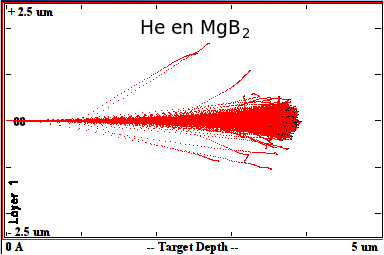
\includegraphics[width=0.5\columnwidth]{Hexy}}\hspace{0.1cm}
 \subfloat[Li en MgB$_2$]{\label{h02}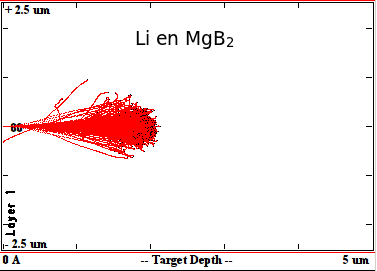
\includegraphics[height=5cm]{Lixy}}
   \caption[Dispersión de iones de He (\ref{h01}) y Li (\ref{h02}) en MgB$_2$]{Dispersión de iones de He (\ref{h01}) y Li (\ref{h02}) en MgB$_2$. Se simuló la colisión de cada uno de los iones en un medio semi infinito de MgB$_2$. A partir de estas simulaciones se estimó que las partículas producidas por la reacción $^{10}\text{B}(n,\alpha)^{7}\text{Li}$ depositan su energía en un volumen $V \, = \, 2.48 \, \mu$m$^3$.}
\label{fig:HeLixy}
\end{figure}

En la Fig.\,\ref{fig:HeLixy} se ven las trayectorias simuladas para cada ion. Los mismos incidían sobre un medio semi-infinito de MgB$_2$ de densidad 2.62\,g/cm$^{3}$\cite{Lui2003}. Esto sería similar a pensar que los productos de la fisión salen en dirección paralela al cable de MgB$_2$. Como el rango de las partículas en el MgB$_2$ es alrededor de 4\,$\mu$m para el He y 2\,$\mu$m para el Li, una conclusión inicial que se puede extraer es que si las partículas salen en dirección perpendicular al cable, la energía depositada en el mismo será muy pequeña, salvo que el ancho y el espesor del cable sean comparables con el rango del He y el Li en MgB$_2$. Sin embargo, más adelante se verá que debido a la dinámica térmica del sistema, el cable de MgB$_2$ debe tener un espesor y un ancho del orden del micrón, ya que de otro modo la señal y la sensibilidad del detector disminuyen drásticamente.

Como primera aproximación al problema se consideró que toda la energía de las partículas se deposita en un único volumen $V_{hs} \, = \, 2.48 \, \mu$m$^3$, y luego se calculó el incremento de temperatura $\Delta T$ que sufre ese volumen de MgB$_2$ como consecuencia de la captura de un neutrón y la reacción nuclear siguiente:
\begin{equation}
  \Delta T \ = \ \frac{Q}{c_p\,V_{hs}\, \delta} \ \approx \ 3.5 \, K
  \label{eq:DT}
\end{equation}
\noindent
donde $Q = 2.3$\,MeV\cite{Nishikawa2008} es la energía liberada en la reacción de captura de un neutrón, $\delta$ es la densidad del MgB$_2$ \cite{Lui2003} y $c_p \ = \ 17$\,J/(kg K) es su calor específico a presión constante \cite{Putti2003} a una temperatura de 39\,K.

La evolución temporal de la temperatura se estudió utilizando un software comercial de simulación por medio del método de elementos finitos (COMSOL MULTIPHYSICS). Se simuló la evolución térmica a lo largo del tiempo de un alambre de MgB$_2$ de 2\,$\mu$m de ancho y con distintos espesores entre 0.2\,$\mu$m y 1.8\,$\mu$m. Se consideró que el mismo se encuentra depositado sobre un sustrato de Si o zafiro de 2\,$\mu$m de espesor, 4\,$\mu$m de ancho y largo igual al del alambre. Los valores de conductividad térmica y calor específico del MgB$_2$ se obtuvieron de \cite{Putti2003} y \cite{Bauer2001}, respectivamente. Los datos análogos del Si se obtuvieron de \cite{Flubacher1959} y de las librerías de propiedades físicas del software COMSOL MULTIPHYSICS. Las propiedades físicas del zafiro también se obtuvieron de las bibliotecas de propiedades del programa COMSOL. En el apéndice \ref{C:tablas} se muestran los datos de entrada empleados en la realización de todas las simulaciones de este trabajo.
\begin{figure}[tbh!]
 \begin{center}
    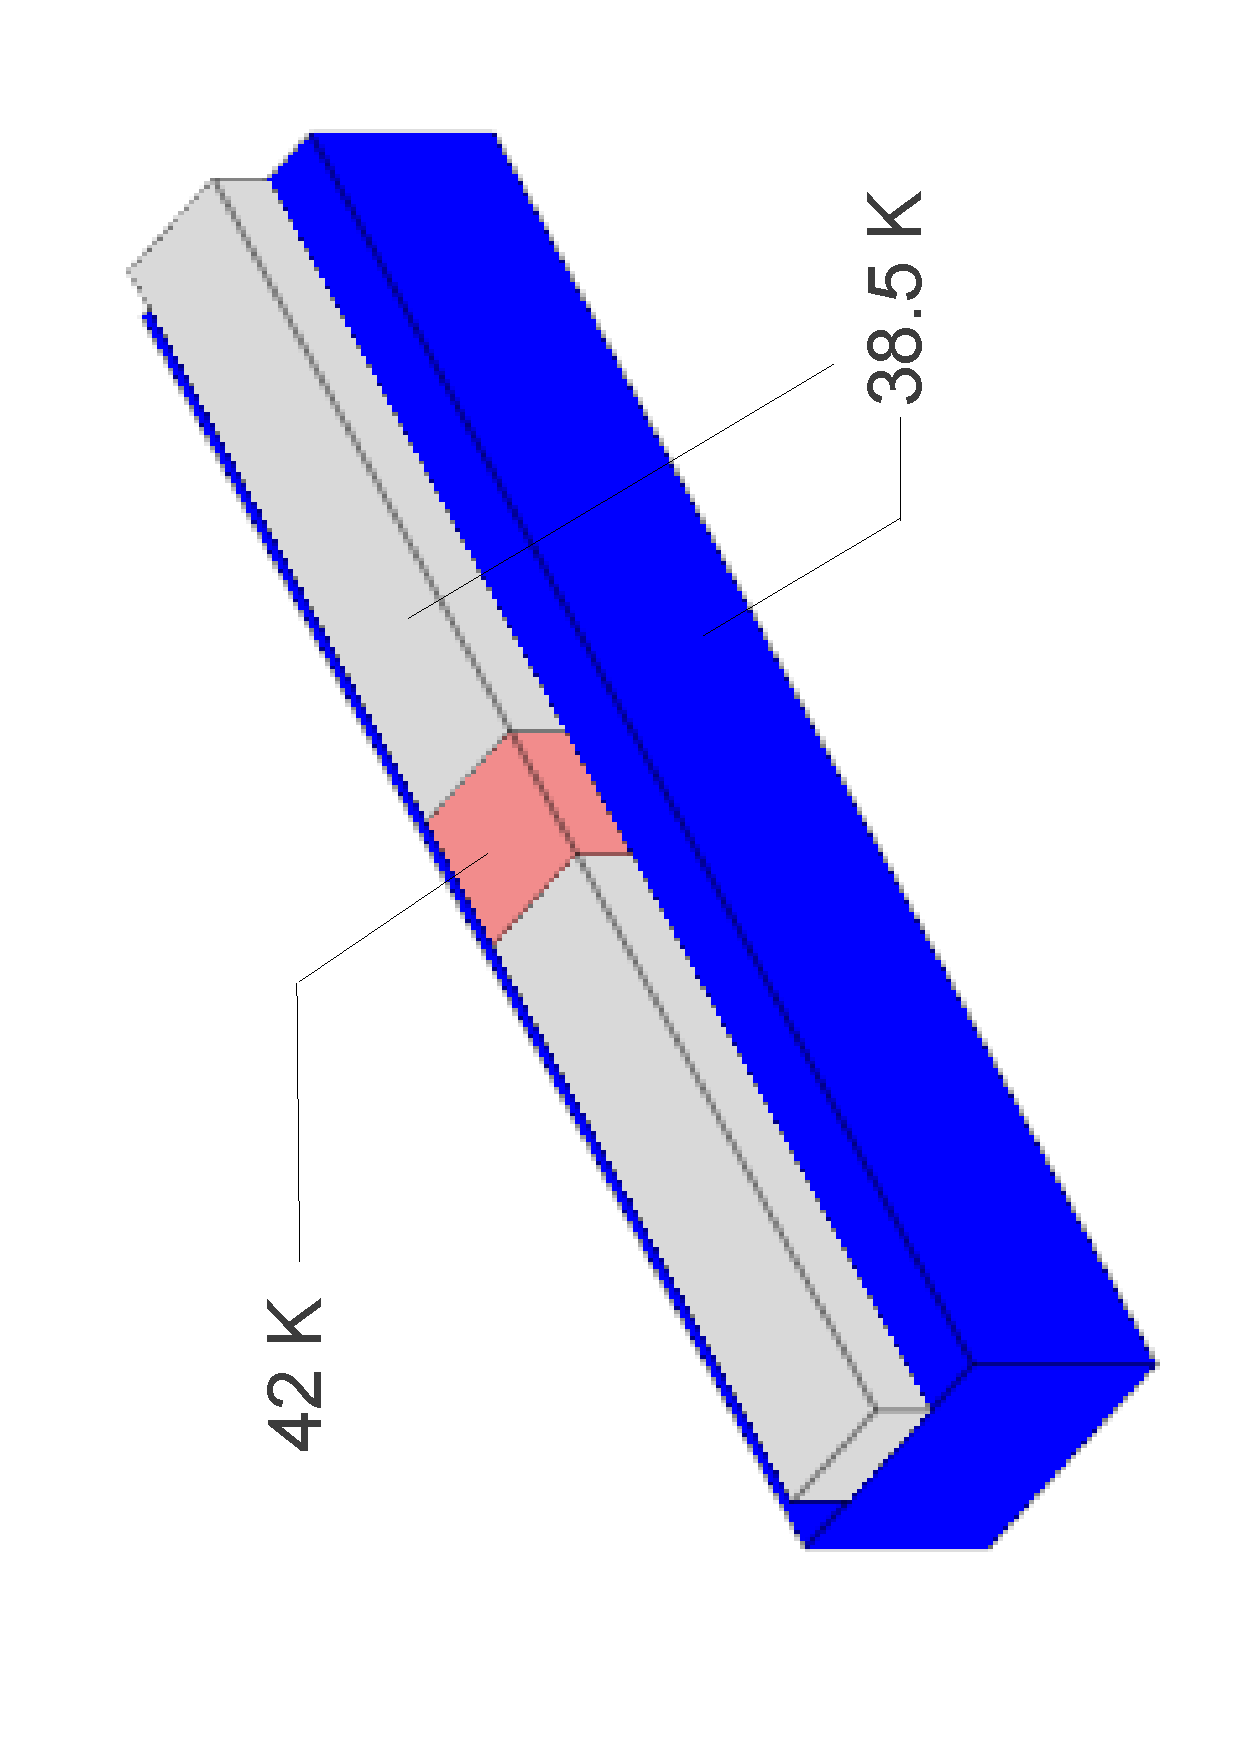
\includegraphics[width=0.45\columnwidth, angle=-90]{sim}
  \end{center}
  \caption[Condiciones de borde utilizadas para simular el comportamiento térmico de un cable de MgB$_2$.]{Se realizó una simulación que consistió en un alambre de MgB$_2$ (gris y rosa) depositado sobre un sustrato que era de silicio o zafiro (azul). Se consideró como condición inicial que todo el sistema estaba a una temperatura de 38.5\,K salvo una porción de 2.48\,$\mu$m$^3$ de volumen (rosa), que se encontraba a 42\,K. Se consideró que la tapa inferior del sustrato se mantenía a temperatura constante e igual a 38.5\,K. El resto del sistema se consideró térmicamente aislado.}
\label{fig:bordes}
\end{figure}

Se consideró una temperatura de operación $T_o \, = \, 38.5$\,K, correspondiente al flanco de la transición superconductora del MgB$_2$\cite{Nagamatsu2001}. Se supuso que el calor se deposita en un volumen $V_{hs}$ y la forma de este volumen cambió de modo que pudiera caber en el alambre (esto es, el volumen se iba haciendo más corto a medida que su espesor aumentaba). Se consideró este criterio con el fin de comparar la variación del tiempo de respuesta del detector para cables de diferentes geometrías que sufren el mismo incremento de temperatura. Un análisis posterior a este tipo de simulaciones mostró que el tiempo de respuesta no se afecta notablemente con la forma y el tamaño que se le asigne a $V_{hs}$. El sistema era lo suficientemente largo como para despreciar cualquier efecto de borde que pudiera aparecer y la condición inicial fue que todo el sistema estaba una temperatura $T_o$, salvo el volumen $V_{hs}$ que tenía una temperatura inicial $T_h \, = \, T_o\, + \, \Delta T$ (Fig.\,\ref{fig:bordes}).

Las condiciones de contorno se impusieron analizando el ambiente de operación del detector. La cara inferior del sustrato fue mantenido a temperatura constante e igual a $T_o$ y se consideró que el resto de las caras estaban aisladas térmicamente del exterior. Esto se hizo así porque el detector va a operar en condiciones de vacío (lo que elimina pérdidas por conducción y convección). Las pérdidas por radiación máximas fueron estimadas a partir de la ecuación de Stefan-Boltzmann\cite{incropera}:
\begin{equation}
\dot{q} \ = \ A\,\sigma \ (T_{detector}^4 \, - \, T_{amb}^4)
\label{eq:sb}
\end{equation}
\noindent
con $\dot{q}$ el flujo saliente de calor, $A$ el área expuesta, $\sigma$ la constante de Stefan-Boltzmann, $T$ la temperatura del detector y $T_{amb}$ la temperatura del medio exterior (considerada como la temperatura de nitrógeno líquido). El flujo de calor por radiación fue comparado con el flujo de calor que existe por conducción a través del MgB$_2$ y del sustrato. Se vio que el flujo de calor por radiación es menor que el flujo por conducción en un factor $10^{7}$, de donde se concluyó que el sistema está térmicamente aislado. Si la temperatura exterior es la ambiente las pérdidas por radiación son menores en un factor $10^{4}$.
\begin{figure}[t!]
 \begin{center}
    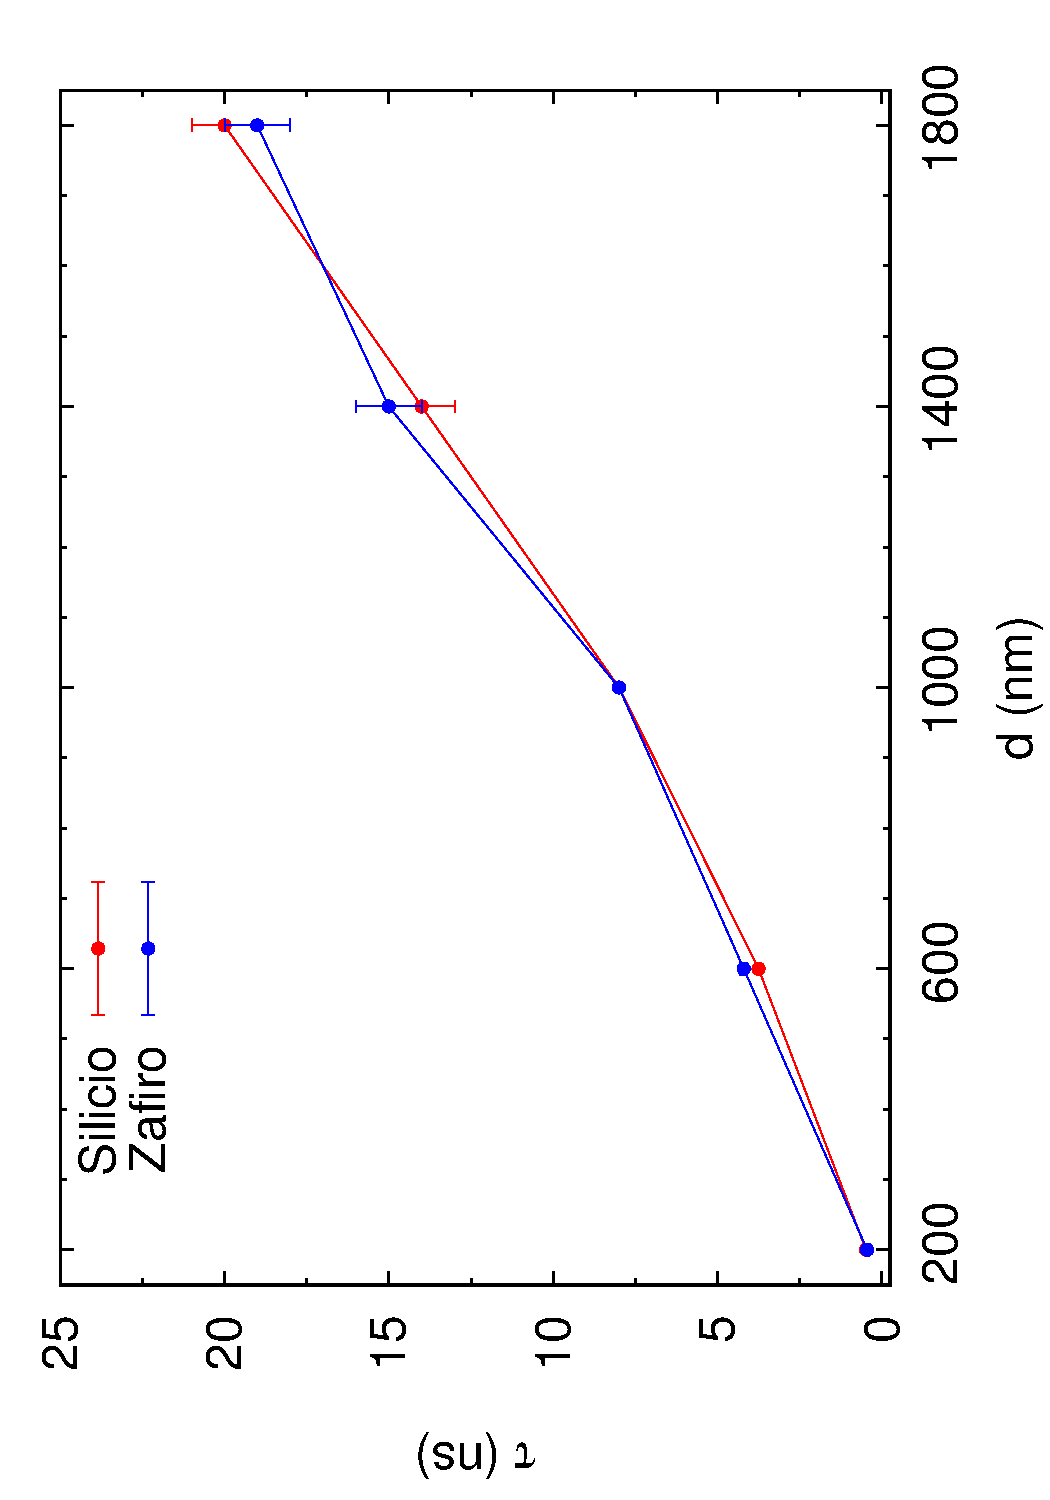
\includegraphics[width=0.55\columnwidth,angle=-90]{tau}
 \end{center}
  \caption[Tiempo de relajación de un cable de MgB$_2$ para diferentes sustratos.]{Tiempo de relajación $\tau$ en función del espesor $d$ de un alambre de MgB$_2$ para diferentes sustratos. Se
concluye de observar la figura que el tiempo de res\-pues\-ta del sistema varía de los pocos nanosegundos a algunas decenas de
nanosegundos para espesores del orden de micrón y que $\tau$ es prácticamente independiente del sustrato utilizado.}
\label{fig:tau}
\end{figure}

Considerando todos estos factores se estudió la evolución temporal de la temperatura del detector y se estimó la variación del tiempo de respuesta $\tau$ del mismo en función de su espesor $d$, como se muestra en la Fig.\,\ref{fig:tau}. Se definió que el sistema había llegado al equilibrio cuando $T_{\text{max}} \, - \, T_o \, \leq \, 0.01$\,K, siendo $T_{\text{max}}$ la temperatura del punto más caliente del detector.

En la Fig. \ref{fig:tau} se observa claramente que el tiempo de respuesta del detector se incrementa en forma lineal con el espesor del film. Esto es razonable, ya que al aumentar el espesor del film, más calor tiene que fluir a través del MgB$_2$ que tiene peor conductividad térmica que el Si y el zafiro. También se puede ver que el tiempo de respuesta del detector es del orden de las decenas de nanosegundos, lo que está en acuerdo con valores obtenidos por otros autores\cite{Nishikawa2008}. Se puede concluir además que el tiempo de respuesta no sufre cambios por depositar el MgB$_2$ en silicio o zafiro.

En la figura\,\ref{fig:cortes} se muestra una secuencia temporal del perfil de temperaturas del detector para diferentes tiempos. Se exhibe la temperatura a lo largo de dos cortes: uno en dirección paralela al alambre y otro transversal al primero, y ambos cortes pasan por el centro del alambre. La figura mostrada corresponde a un cable de MgB$_2$ de 15\,$\mu$m de largo, 2\,$\mu$m de ancho y 0.8\,$\mu$m de espesor, depositado sobre un sustrato de Si.
\begin{figure}[tbh!]
 \begin{center}
    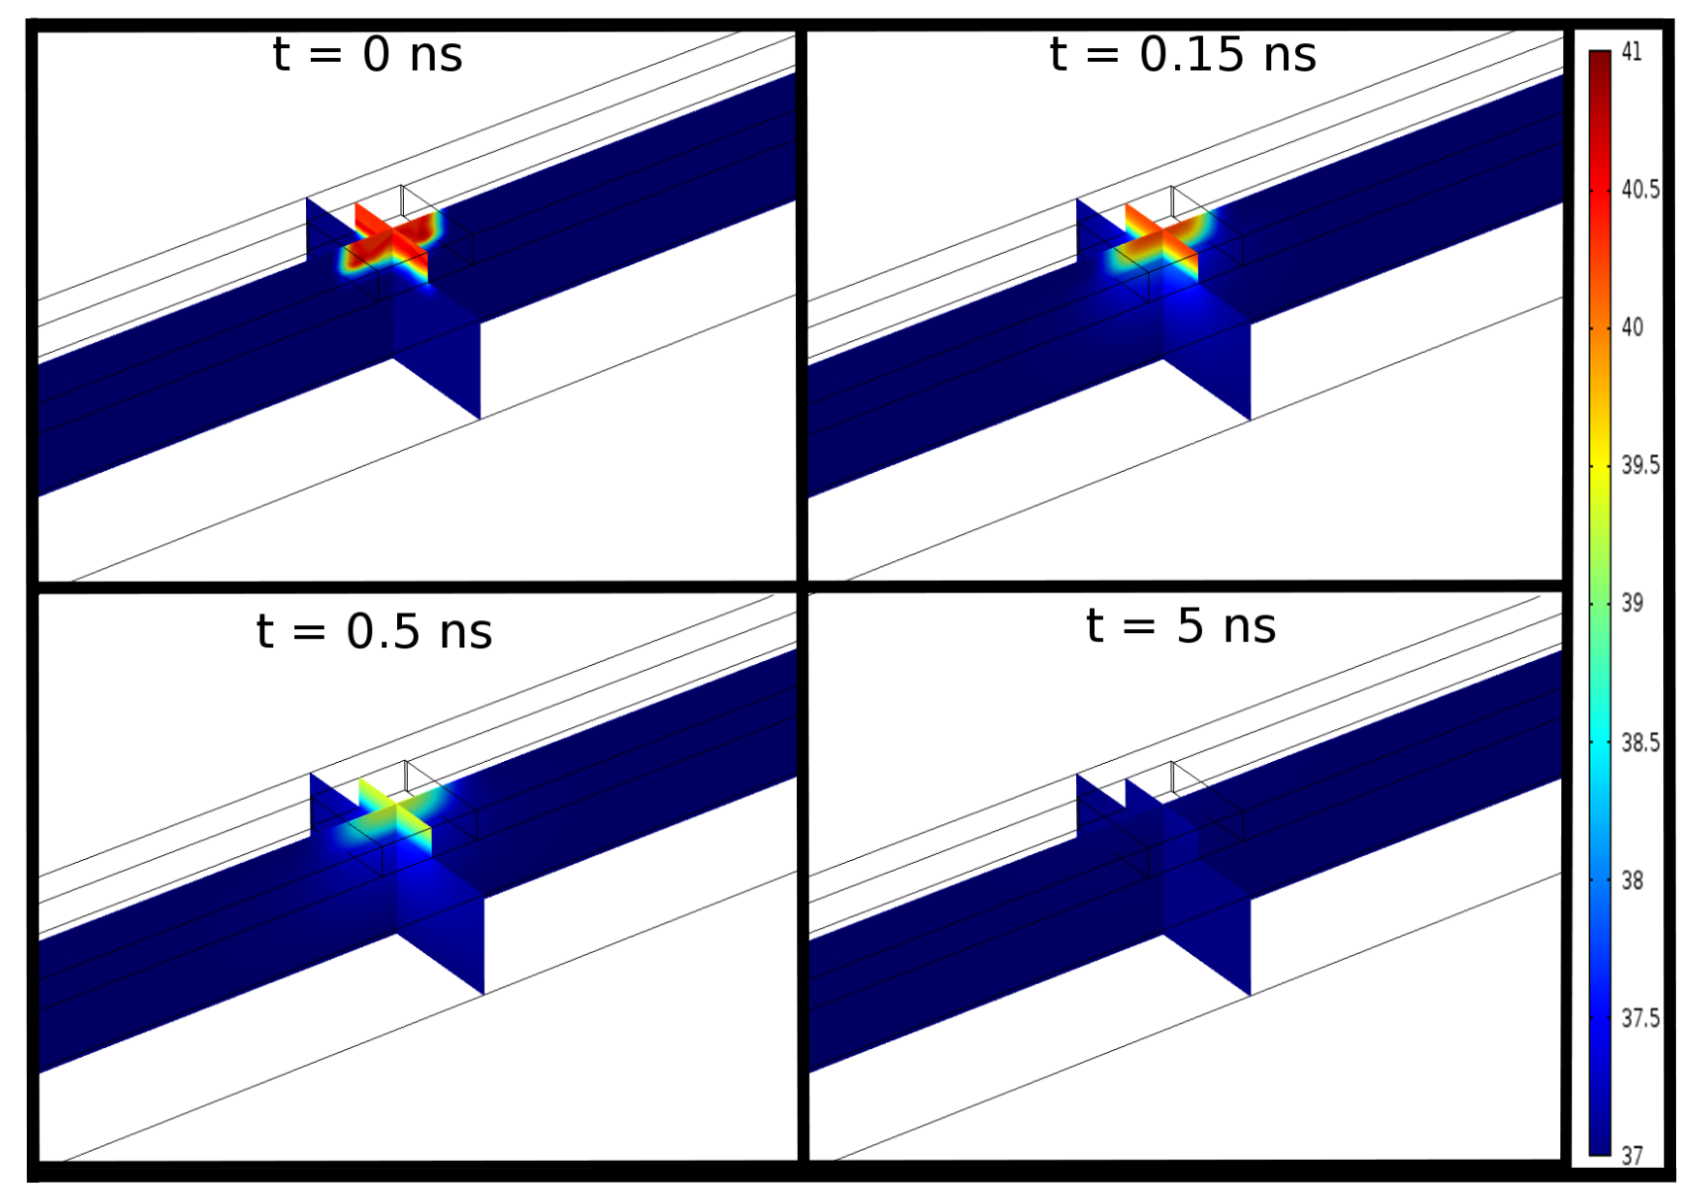
\includegraphics[width=0.95\columnwidth,angle=0]{relax}
  \end{center}
  \caption[Temperatura del detector para diferentes tiempos.]{Temperatura del detector para diferentes tiempos. Se muestra un alambre de MgB$_2$ de 15\,x\,2\,x\,0.8\,$\mu$m depositado sobre un sustrato de Si de 15\,x\,4\,x\,2\,$\mu$m.}
\label{fig:cortes}
\end{figure}

Se aprecia que la región más caliente del detector es siempre la misma, es decir, parece ser que el calor tiende a difundir mucho más a través del sustrato que dentro del MgB$_2$. Teniendo en cuenta que la conductividad térmica del silicio es $\kappa_{\text{Si}}\,=\,3510$\,W/(m\,K) y la del MgB$_2$ es $\kappa_{\text{MgB}_2}\,=\,14.35$\,W/(m\,K)\cite{Glassbrenner1964,Bauer2001}, parece razonable que sea así. Resultados similares se obtuvieron al reemplazar el sustrato del Si con zafiro, lo cual también tiene sentido ya que $\kappa_{\text{zafiro}}\,=\,12000$\,W/(m\,K)\cite{Ekin2006}.
\nomenclature{$d$}{Espesor de un film o cable.}
\nomenclature{$l$}{Longitud de un cable.}
\nomenclature{$a$}{Ancho de un cable.}
\nomenclature{$\kappa$}{Conductividad térmica.}
\nomenclature{$c_p$}{Calor específico a presión constante.}
\nomenclature{$A$}{Área del detector.}
\nomenclature{$V_{hs}$}{Volumen en que se deposita la energía de una reacción.}
\nomenclature{$\delta$}{Densidad de un material.}
\nomenclature{$\rho$}{Resistividad de un material.}
\nomenclature{$T_{hs}$}{Temperatura que alcanza el volumen en donde se deposita la energía de la reacción.}
\nomenclature{$T_o$}{Temperatura de operación del detector.}
\section{Señal del detector}\label{S:signal}
Como se dijo antes, el atributo característico de los detectores TES es que obtienen una muy buena señal al aprovechar los cambios abruptos de la resistividad de un film superconductor. El propósito de esta sección es estimar la señal producida por un detector de MgB$_2$ al capturar un neutrón y calcular la temperatura óptima de operación del dispositivo, definida como aquella en que la variación de la resistencia producida por la captura de un neutrón sea máxima. En lo que sigue, los términos señal y variación de la resistencia se utilizarán como sinónimos, ya que la señal emitida por el detector es proporcional a la variación de la resistencia del MgB$_2$.

Se estudió la variación de la resistencia $\Delta R$ en el volumen $V_{hs}$ en función de la temperatura inicial del mismo. Para este estudio se consideró un modelo diferente al de la sección anterior, es decir, se consideró que el volumen $V_{hs}$ tiene ancho y espesor iguales a los del cable de MgB$_2$, pero para este modelo se consideró una longitud fija. El cambio en la resistencia del alambre $\Delta R$ se calculó a partir de la relación\cite{Sears1964}:
\begin{equation}
  \Delta R \ = \ \frac{\Delta \rho \ l}{a \ d}
  \label{eq:DR}
\end{equation}
\noindent
siendo $l$, $a$ y $d$ la longitud, el ancho y el espesor del volumen $V_{hs}$, respectivamente. Se tomaron valores de $a \, = \, 2\,\mu$m, $0.2\, \mu m \, \leq \, d \, \leq \, 1\,\mu$m y $l \, = \, 2\,\mu$m. La variación de $\rho$ en función de la temperatura se obtuvo a partir las mediciones obtenidas de \cite{Nagamatsu2001} y que se ven en la Fig.\,\ref{fig:rovsT}.
\begin{figure}[tbh!]
 \begin{center}
    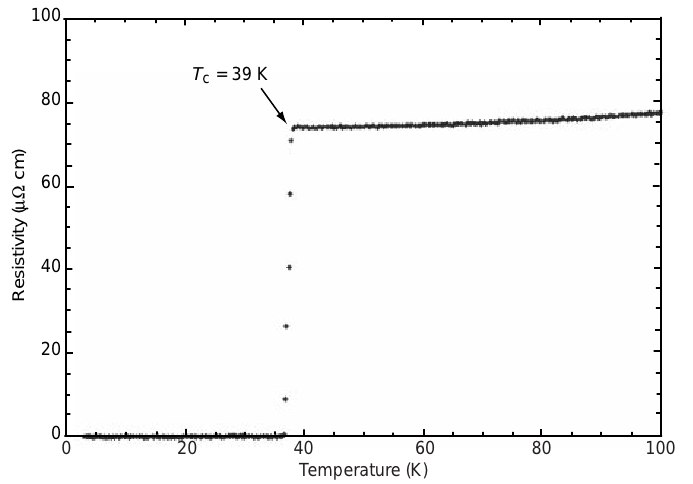
\includegraphics[width=0.75\textwidth]{rovsT}
  \end{center}
  \caption[Variación de la resistividad del MgB$_2$ en función de la temperatura.]{Variación de la resistividad del MgB$_2$ en función de la temperatura. Puede verse el cambio abrupto en la resistividad del MgB$_2$ a 39 K. Imagen obtenida de \cite{Nagamatsu2001}.}
\label{fig:rovsT}
\end{figure}

En la Fig. \ref{fig:rvsT} se muestra como varía la señal del alambre de MgB$_{2}$ en función de la temperatura inicial, comparando el resultado para diferentes espesores. Puede observarse que el cambio en la señal es del orden de algunos Ohm y que la misma decrece fuertemente a medida que el cable se vuelve más grueso. También puede apreciarse que incrementar el espesor del cable obliga a tener un control más estricto de la temperatura. Dicha conclusión es razonable dentro del modelo propuesto, ya que un espesor menor implica que la misma energía de la reacción se deposita en una región de material que es más pequeña. Esto trae aparejado que el incremento de temperatura sea mayor, lo que simplifica el control de la misma.
\begin{figure}[tbh!]
 \begin{center}
    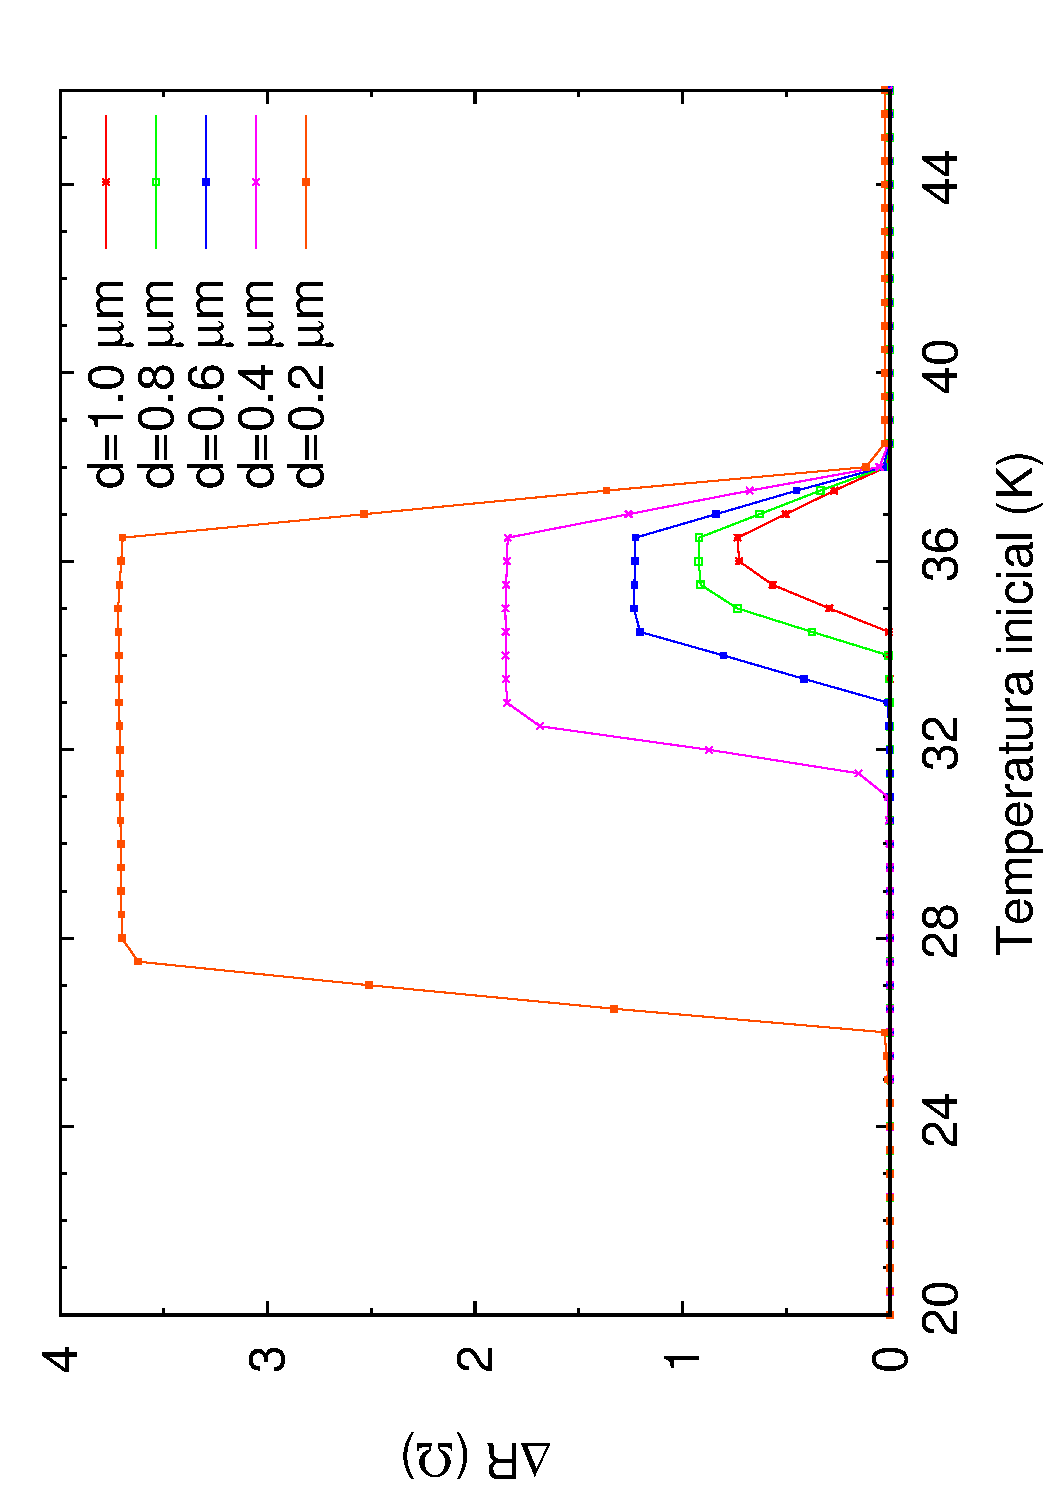
\includegraphics[width=0.5\textwidth, angle=-90]{rvst}
  \end{center}
  \caption[Variación de $\Delta$R en función de la temperatura inicial del MgB$_2$.]{Variación de $\Delta$R en función de la temperatura inicial del MgB$_2$. Las dimensiones de la porción de MgB$_2$ eran  2\,$\mu$m\,x\,2\,$\mu$m\,x\,$d$\,nm.}
\label{fig:rvsT}
\end{figure}
%\newpage

Sin embargo, es válido preguntarse si es correcto pensar que la energía que se deposita en el cable es independiente de las dimensiones del mismo, ya que si el cable se vuelve más delgado los iones escaparían del mismo antes de depositar toda su energía en el MgB$_2$. Siguiendo esta motivación se realizaron simulaciones estudiando el cambio en la señal disminuyendo la energía que se deposita en el detector. El volumen $V_{hs}$ se modeló de la misma forma que en el cálculo anterior, considerando solamente alambres de 200\,nm y 800\,nm de espesor, como se puede ver en la Fig. \ref{fig:RvsrvsQ}. 

\begin{figure}[h!]
 %\centering
  \hspace{-1.4cm}
 \subfloat[200\,nm]{\label{fig:R1}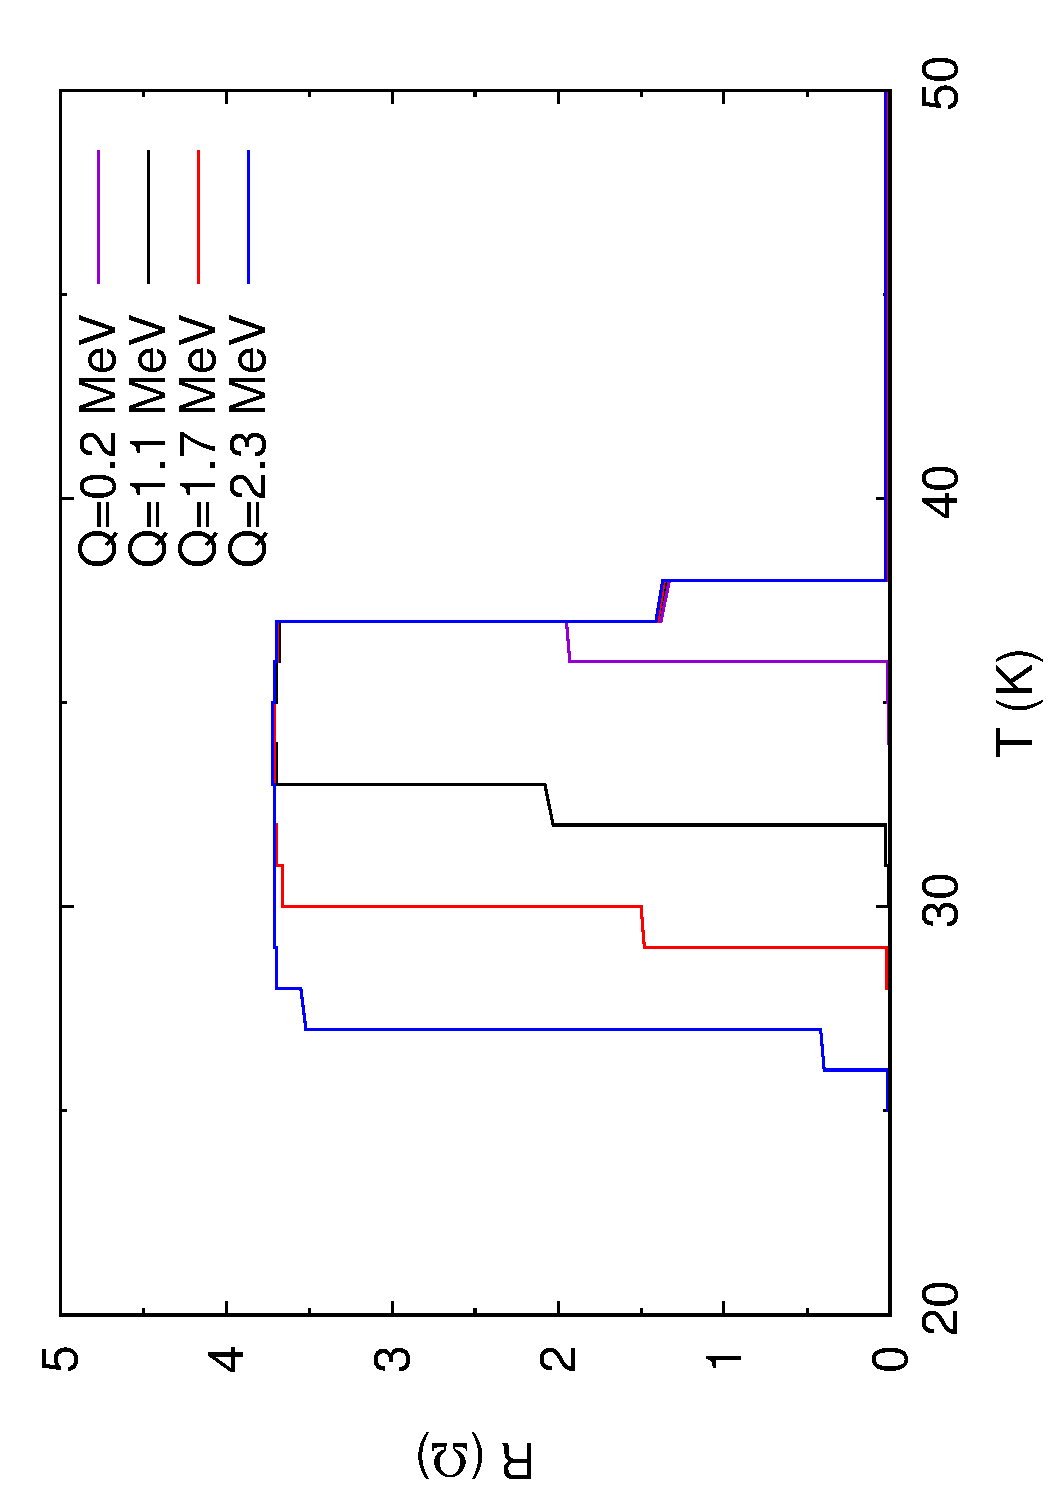
\includegraphics[width=0.4\columnwidth,angle=-90]{RvsTvsQ_200nm}}
 \subfloat[800\,nm]{\label{fig:R2}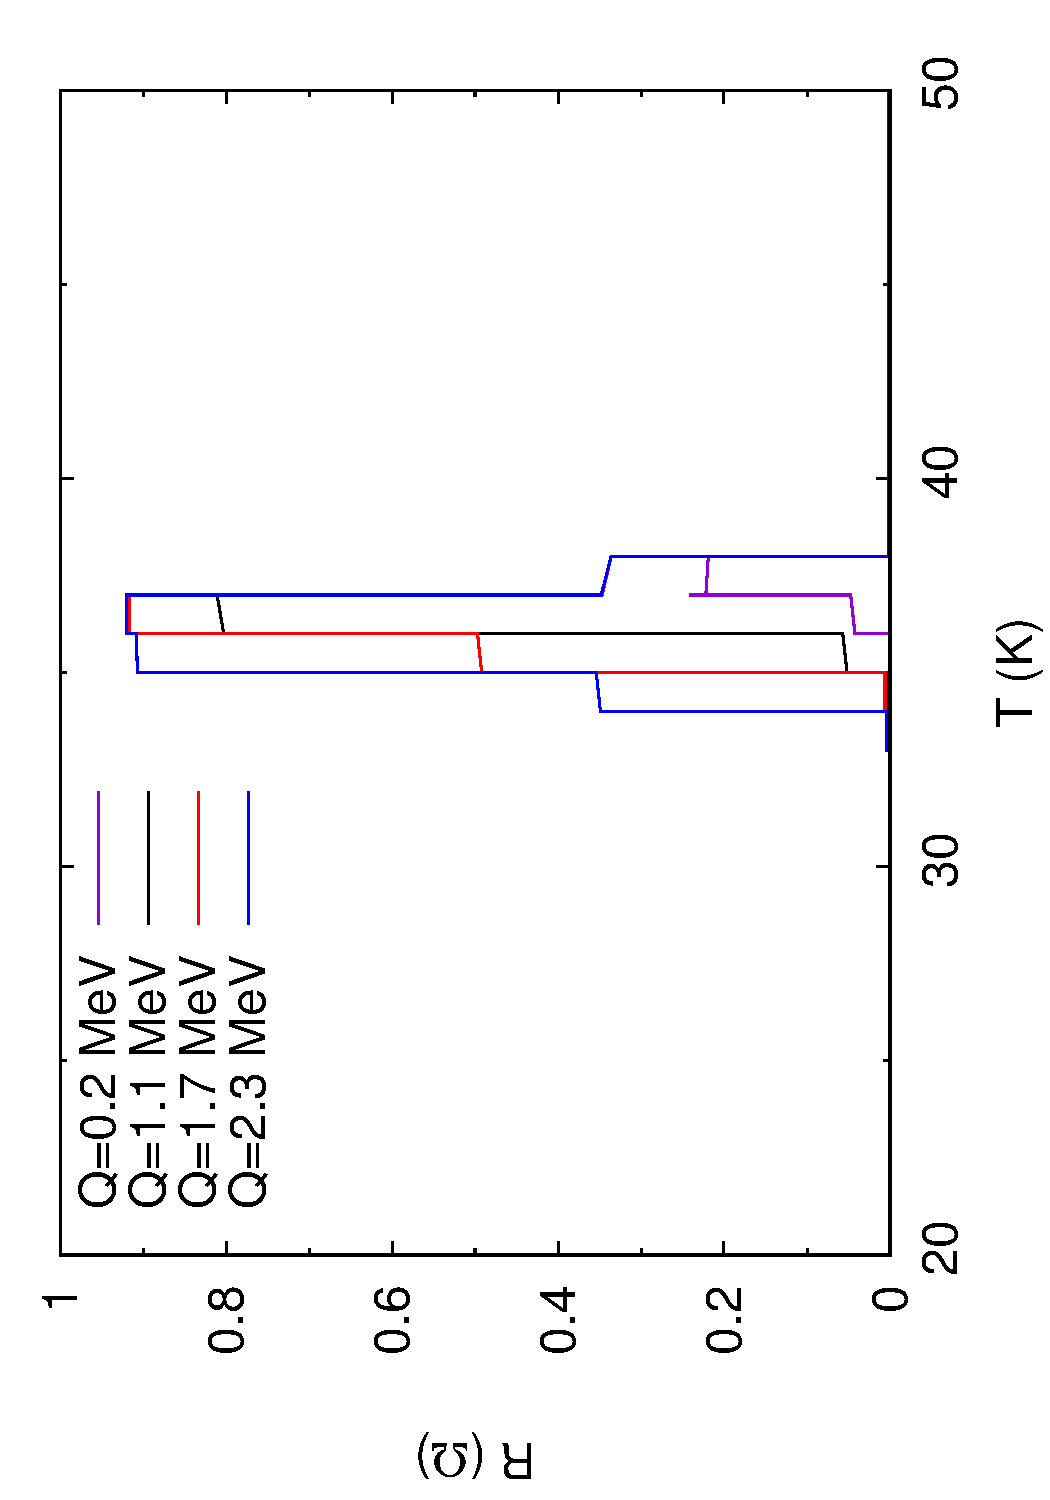
\includegraphics[width=0.4\columnwidth,angle=-90]{RvsTvsQ_800nm}}
   \caption[Señal producida por el detector en función de la temperatura de operación y la energía depositada en el mismo.]{Señal producida por el detector en función de la temperatura de operación y la energía depositada en el mismo. En la Fig. \ref{fig:R1} se muestra el cálculo realizado para un cable de un espesor de 200\,nm mientras que en la \ref{fig:R2} aparece el resultado para un cable de 800\,nm. A partir de comparar estos gráficos es claro ver que un cable delgado produce una mayor señal que uno más grueso, incluso si en el cable delgado se deposita una energía diez veces menor que en el grueso.}
\label{fig:RvsrvsQ}
\end{figure}

%\newpage
Con los datos de la Fig. \ref{fig:RvsrvsQ} junto con los análisis hechos previamente se puede hacer un estudio más integral de las ventajas y desventajas de las diferentes geometrías del detector. Por ejemplo, en la Fig. \ref{fig:R1} puede verse que si el espesor del cable de MgB$_{2}$ es de 200\,nm se tiene una señal que es mayor que la que se puede esperar para un alambre de 800\,nm, incluso si en el cable se deposita una energía diez veces menor. En ese sentido, la misma conclusión puede extraerse si la variable a analizar es la temperatura óptima de operación del detector, ya que de comparar las Figs. \ref{fig:R1} y \ref{fig:R2}, puede verse que el intervalo en que se observa un máximo de señal para un film de espesor de 200\,nm, es siempre igual o mayor al intervalo esperado para un film de 800\,nm, sea cual sea la energía que se deposita en el detector.
\section{Acoplamiento térmico-eléctrico}\label{S:termyelec}
En las secciones anteriores se estudió por un lado como se enfría una sección de MgB$_2$ sobre un sustrato que se mantiene a una temperatura fija. Por otro lado se mo\-de\-ló y calculó también la modificación de la resistencia de un cable de MgB$_2$ como resultado de la captura de un neutrón. Si se observa con un poco de cuidado, puede verse que en un cable de MgB$_2$ diseñado adecuadamente aparecen dos fenómenos interesantes. El primero es el ''efecto fusible'', es decir que la diferencia de tensión en los extremos de un cable se incrementa súbitamente debido a la reacción que se inicia con la absorción de un neutrón. El segundo es que debido a que una porción importante del material deja de ser superconductor, el mismo se convierte en una fuente de calor, debido al efecto Joule. Este acoplamiento que ocurre entre el sistema térmico y el eléctrico, puede considerarse despreciable si las corrientes circulantes son lo suficientemente bajas. Sin embargo, debido al comportamiento altamente no lineal que tiene la resistividad del MgB$_2$ alrededor de la transición superconductora, es razonable preguntarse qué tan baja debe ser la corriente circulante para ser considerada despreciable. De aquí se concluye que hacer un estudio acoplando el problema térmico y el eléctrico resulta necesario si se quieren determinar las condiciones de operación óptimas del detector. Además, la inclusión de una fuente de calor en el problema podría modificar el tiempo de respuesta del detector, detalle que puede ser importante si se busca un equipo que trabaje con elevados flujos de neutrones.

En este punto parece apropiado comentar algunas de las complicaciones que aparecen cuando se busca resolver un problema que se representa por un sistema de ecuaciones diferenciales acopladas (la ecuación de transferencia del calor y la de los circuitos de corriente continua). Este acoplamiento puede resultar complicado, sobre todo si el mismo se hace a través de una variable que tiene un comportamiento no lineal, como lo es la resistencia del MgB$_2$ en este caso. Los mayores problemas que aparecen son la aparición de inestabilidades, oscilaciones, soluciones espurias y que el programa falle en poder satisfacer las condiciones de borde exigidas. Luego de algún trabajo y estudio del programa utilizado para hacer las simulaciones, se encontró que la mejor forma de solucionar estos problemas es la siguiente: primero se resuelve el problema eléctrico para la condición inicial (tal como fue planteada en la sección \ref{S:term}) sin tener en cuenta la evolución temporal del sistema. Una vez logrado esto se toman los datos (corrientes y tensiones) de esta simulación y se los utiliza como condición inicial del problema térmico-eléctrico dependiente del tiempo.

En adición a las simulaciones que permitieron estimar el tiempo de respuesta, se llevó a cabo una simulación más para estimar las dimensiones mínimas que debe tener el detector para que pueda detectar neutrones eficientemente. En este caso se consideró un bloque de MgB$_2$ que se encuentra en estado superconductor. Se supuso que la captura de un neutrón causó una supresión del parámetro de orden superconductor en un cubo de 0.2\,$\mu$m de lado\cite{Machida2004}. Por lo tanto se consideró que la energía de la reacción se depositó inicialmente en ese volumen. Se puso al bloque de MgB$_2$ en contacto directo con una fuente térmica fría, y se lo conectó a una fuente eléctrica de corriente continua. El objetivo de esta simulación era ver el tamaño máximo que adquiría la región normal, es decir, no superconductora, del MgB$_2$.
\begin{figure}[h!]
 \begin{center}
    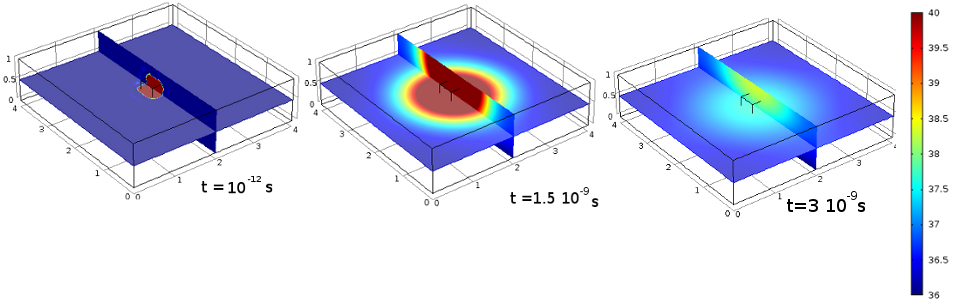
\includegraphics[width=\columnwidth]{secuencia3}
  \end{center}
  \caption[Secuencia temporal que indica como fluye el calor desde el ''punto caliente'' inicial hacia el resto del material.]{Secuencia temporal que indica como fluye el calor desde el ''punto caliente'' inicial hacia el resto del material. Se muestran dos cortes transversales del bloque de MgB$_2$ simulado. La parte inferior del bloque se mantuvo a 36\,K. El espesor del bloque era de 1\,$\mu$m. Puede verse como la región del material que se vuelve normal tiene un tamaño máximo del orden de 1\,$\mu$m antes de empezar a hacerse más pequeña.}
\label{fig:secuencia}
\end{figure}

Así como se hizo en la sección \ref{S:term}, el estudio del acoplamiento de los problemas térmico y eléctrico también se hizo utilizando el software comercial COMSOL MULTIPHYSICS. Se consideró como ecuación constitutiva $\mathbf{J} \, = \, \sigma(T) \, \mathbf{E}$ y se incorporó la disipación debida al efecto Joule ($\dot{q} \, = \, J^2/\sigma$). La conductividad eléctrica $\sigma(T)$ se obtuvo de la curva de resistividad de una muestra bulk de MgB$_2$ que se muestra en la Fig \ref{fig:rovsT}, al igual que en la sección \ref{S:signal}. En la Fig. \ref{fig:secuencia} se pueden apreciar dos cortes perpendiculares que muestran el campo de temperaturas en el bloque de MgB$_{2}$ en distintos momentos de la simulación: el instante inicial, el instante en el que la región normal ocupó el máximo volumen y un instante posterior en que el sistema estaba prácticamente en equilibrio térmico. A partir de estas imágenes se puede observar que la región normal adquiere una forma esférica cuyo radio máximo es un poco mayor que un micrón y que luego empieza a hacerse más pequeño. Esto implica que un cable de MgB$_2$ cuyo ancho y espesor sean mucho mayores que un micrón no detectará eficientemente la captura de un neutrón, ya que es altamente probable que incluso en el momento en que la región normal tome su tamaño máximo, aún exista un paralelo superconductor por el que circulará la mayoría de la corriente aplicada. Un análisis similar al previo se hizo reduciendo el espesor del bloque de MgB$_2$ a 0.5\,$\mu$m y 0.2\,$\mu$m. Se pudo apreciar que si bien el tiempo de relajación del sistema disminuye, el tamaño máximo de la región normal aún es del orden de un micrón. La conclusión que se puede hacer entonces concuerda con la extraída de las secciones \ref{S:term} y \ref{S:signal}, y es que para poder tener una buena sensibilidad ante la captura de un neutrón, es necesario que tanto el espesor del cable como su ancho sean de dimensiones del orden o inferiores al micrón.
\nomenclature{$\sigma$}{Conductividad eléctrica.}

También se estudió el comportamiento de las simulaciones de la sección \ref{S:term} agregando la componente eléctrica del problema. Las condiciones de contorno para la parte térmica de la simulación eran las mismas que las que se utilizaron para la sección \ref{S:term}. Se trabajó en el problema eléctrico suponiendo que el detector operaba tanto a corriente constante como a tensión constante.
\subsection{Simulaciones a corriente constante}\label{ss:Icte}
Se hicieron simulaciones a diferentes corrientes en el rango de 1\,$\mu A$ y 100\,$m A$ para espesores de 200\,$nm$ y 1000\,$nm$, y se estudió la diferencia de potencial entre los extremos del alambre, así como la variación de la temperatura del mismo en función del tiempo.

A partir de las simulaciones se encontró que existe una corriente a partir de la cual la temperatura del sistema no tiende asintóticamente a la inicial, lo cual es lógico, ya que si la disipación Joule produce suficiente calor como para mantener la temperatura del cable por encima de $T_c$, el sistema nunca vuelve al estado superconductor, ya que el MgB$_2$ nunca se enfría lo suficiente como para que la resistividad empiece a disminuir. El valor de esta corriente umbral depende de la forma del alambre de MgB$_2$ pero para las geometrías simuladas se encontró que tiene un valor que está entre la decena y la centena de miliamperes. 
\begin{figure}[h!]
 \begin{center}
    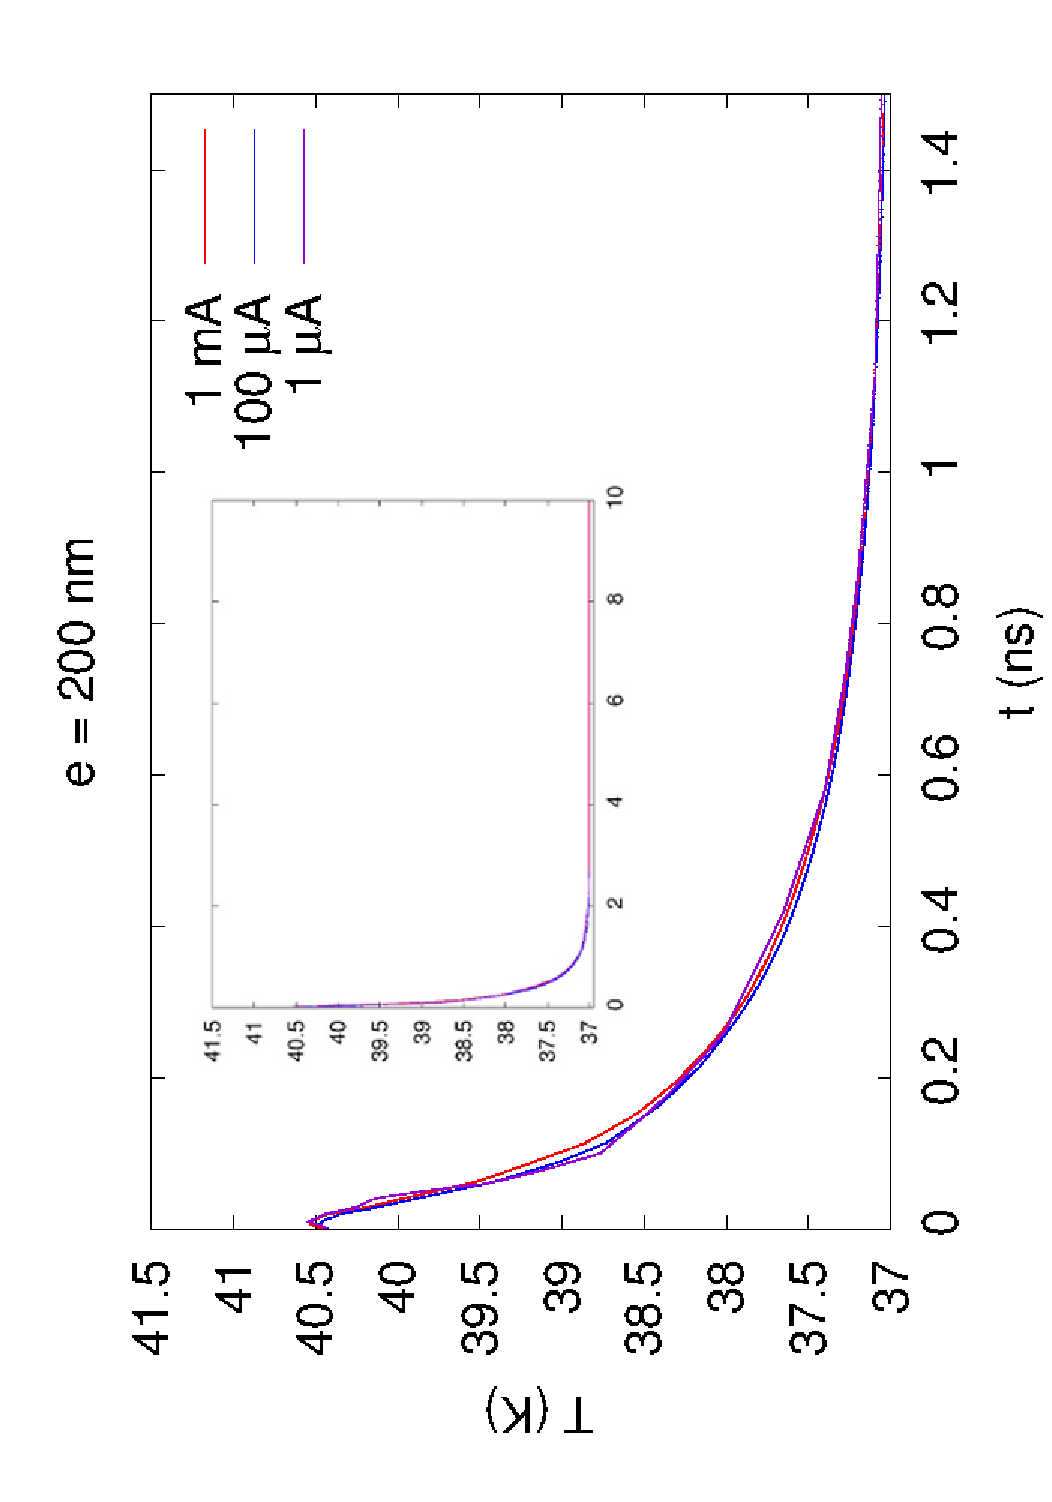
\includegraphics[width=0.5\columnwidth, angle=-90]{TvstxI}
  \end{center}
  \caption[Temperatura en función del tiempo para un alambre de MgB$_2$ de 200\,$nm$ espesor y con diferentes corrientes circulantes.]{Temperatura en función del tiempo para un alambre de MgB$_2$ de 200\,$nm$ espesor y con diferentes corrientes circulantes. Se observa que el tiempo de relajación es prácticamente independiente de la corriente circulante.}
\label{fig:TvstxI}
\end{figure}

Por otro lado, si la corriente que circula por el MgB$_2$ está por debajo de este umbral, el tiempo de relajación del sistema parece ser independiente de la misma, como se puede ver en la Fig. \ref{fig:TvstxI}. Además, en la Fig. \ref{fig:TvstxexI} se aprecia que no existe una diferencia significativa en el tiempo de relajación cuando se desacopla el problema eléctrico del térmico. De aquí puede concluirse que en el régimen estable el calentamiento debido al efecto Joule no juega un rol significativo en la dinámica del sistema.

\begin{figure}[h!]
 \begin{center}
    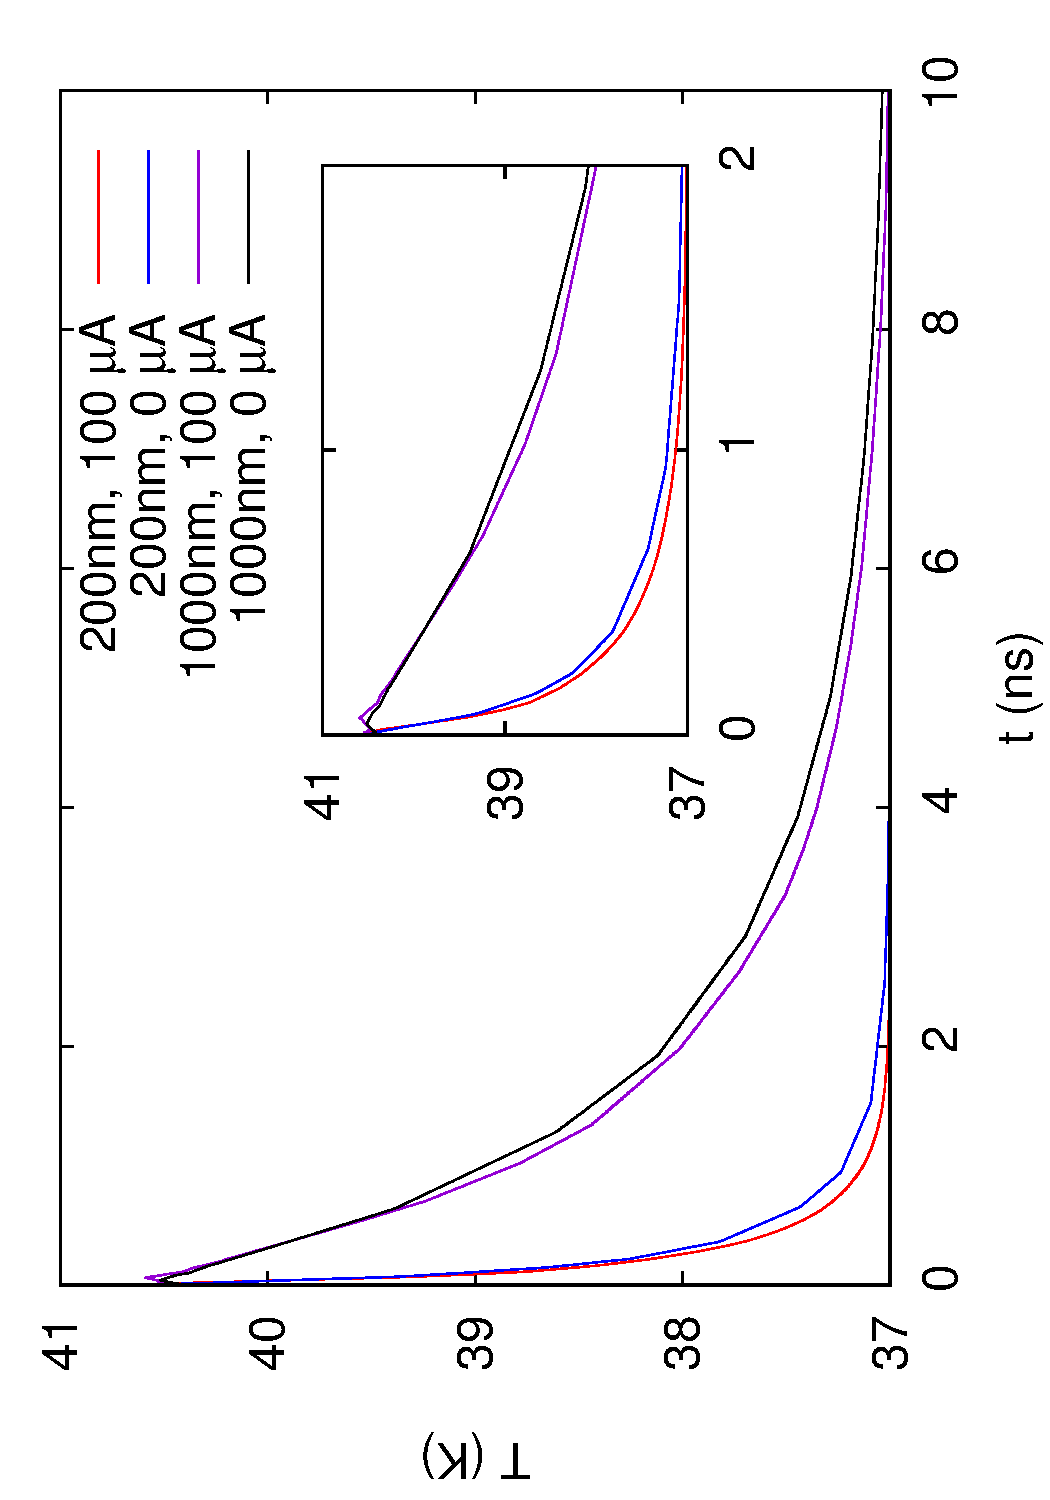
\includegraphics[width=0.5\columnwidth, angle=-90]{TvstxexI}
  \end{center}
  \caption[Comparación del tiempo de relajación para un alambre de MgB$_2$ para el caso desacoplado y acoplado.]{Comparación del tiempo de relajación para un alambre de MgB$_2$ para el caso desacoplado (corriente 0) y acoplado. No se observan diferencias apreciables entre los dos casos.}
\label{fig:TvstxexI}
\end{figure}

Por último se estudió cómo varía la señal del detector en función del tiempo, para lo cual se graficó la evolución temporal de la resistencia del alambre de MgB$_2$. En la figura \ref{fig:signal} se compara además cómo varía la respuesta para cables de diferentes espesores. Puede verse como al aumentar el espesor del alambre el pico de la señal se vuelve más ancho y de menor altura. 
\begin{figure}[h!]
 \begin{center}
    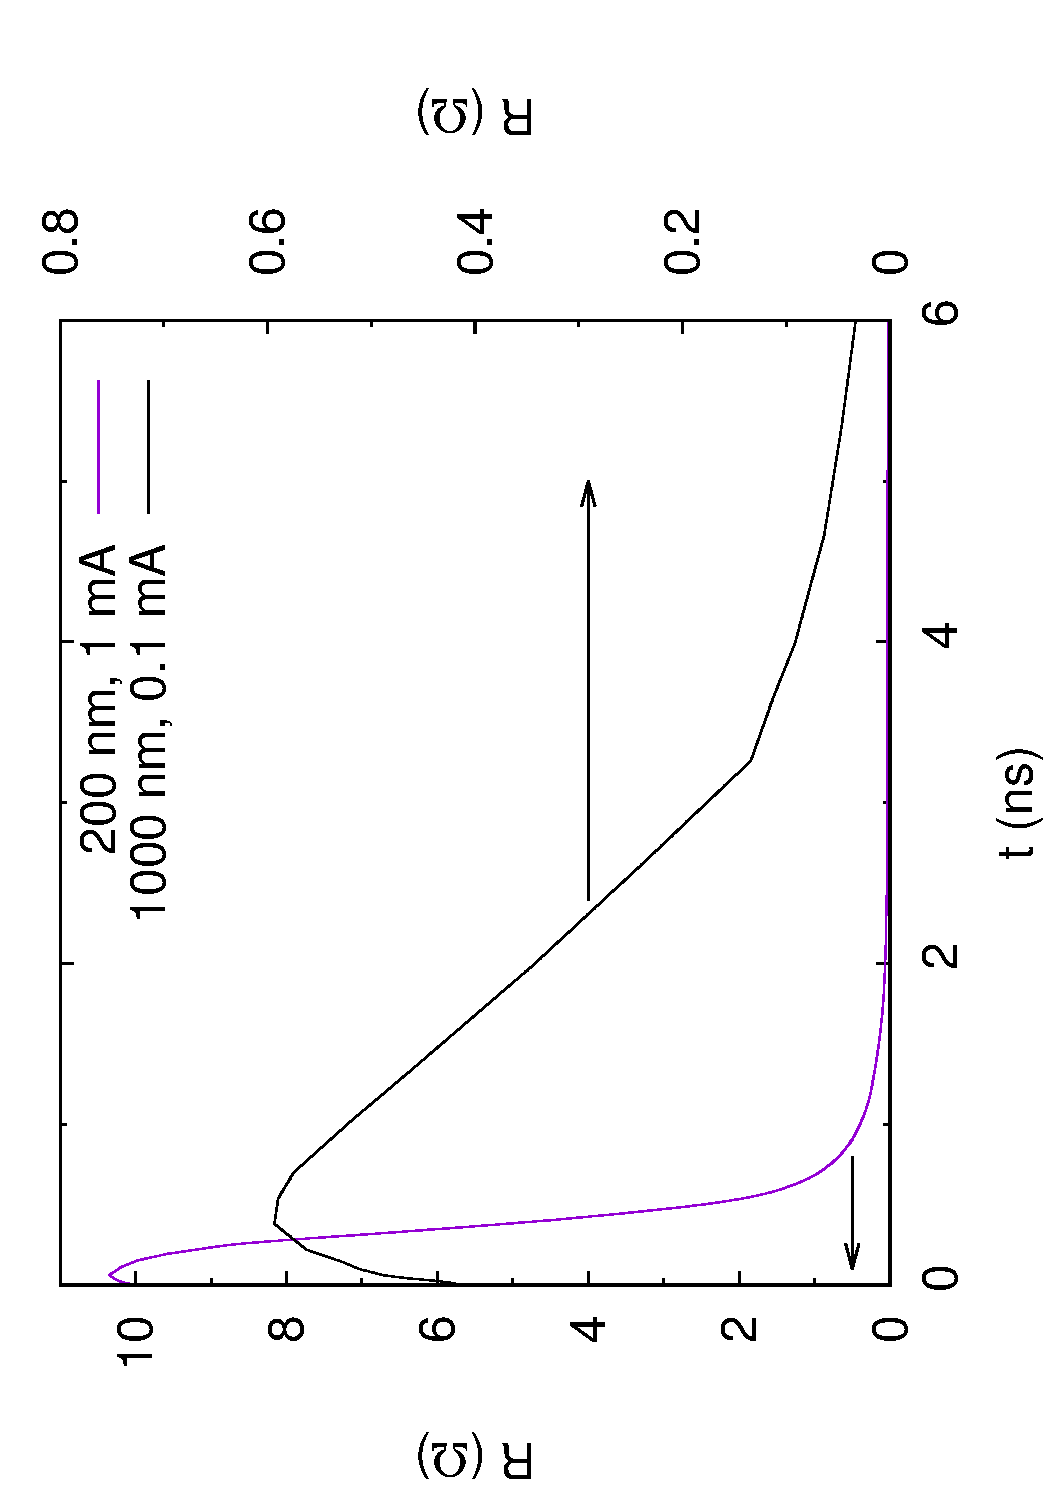
\includegraphics[scale=0.55, angle=-90]{signal}
  \end{center}
  \caption[Resistencia en función del tiempo de dos alambres de MgB$_2$, uno de 1000 nm de espesor y otro de 200 nm de espesor.]{Resistencia en función del tiempo de dos alambres de MgB$_2$, uno de 1000 nm de espesor y otro de 200 nm de espesor. El resto de las dimensiones son equivalentes. Se observa que los pico de resistencia se vuelven más anchos y más bajos a medida que aumenta el espesor del alambre.}
\label{fig:signal}
\end{figure}

En la sección \ref{S:eficiencia} se mostrará la dependencia de la eficiencia del detector con el espesor del mismo.  Allí se muestra que la probabilidad de captura de un neutrón es proporcional al espesor del detector. Esto es, si el espesor del detector se incrementa en un factor 5, también lo hace la probabilidad de captura. En la Fig. \ref{fig:signal} puede verse que un incremento en un factor 5 de la eficiencia redunda en un detrimento en un factor 10 en el valor de la señal. También implica un notable alargamiento en el tiempo de respuesta, lo que puede ser deseable en función de la electrónica de seguimiento que se disponga. Sin embargo, esto también se puede lograr a partir de crecer el detector en una estructura tipo membrana, de lo que se concluye finalmente que no es recomendable buscar un mayor espesor del detector, puesto que la ganancia en eficiencia no parece compensar los aspectos negativos asociados a un detector de mayor volumen.
\subsection{Simulaciones a tensión constante}\label{ss:Vcte}
En la sección \ref{S:tes} se explicó que si un TES se  opera a tensión constante, se puede utilizar el efecto Joule como mecanismo de control de la temperatura de operación del detector. Para lograr esto, es necesario que la temperatura de la fuente fría se encuentre muy por debajo de la $T_c$ del material que se usa como volumen de detección. Cabe mencionar que los dispositivos en los que este mecanismo se implementa con éxito son aquellos materiales que tienen una transición superconductora a temperaturas del orden de los cientos de milikelvin. El propósito de esta sección es estudiar la viabilidad de implementar un control de temperatura utilizando únicamente el efecto Joule como señal de realimentación. El poder lograr esto sería extremadamente conveniente, ya que en ese caso se evita la necesidad de incorporar equipos extra para realizar un control de la temperatura, simplificando así la construcción del dispositivo.
 \begin{figure}[tbh!]
   \begin{center}
	 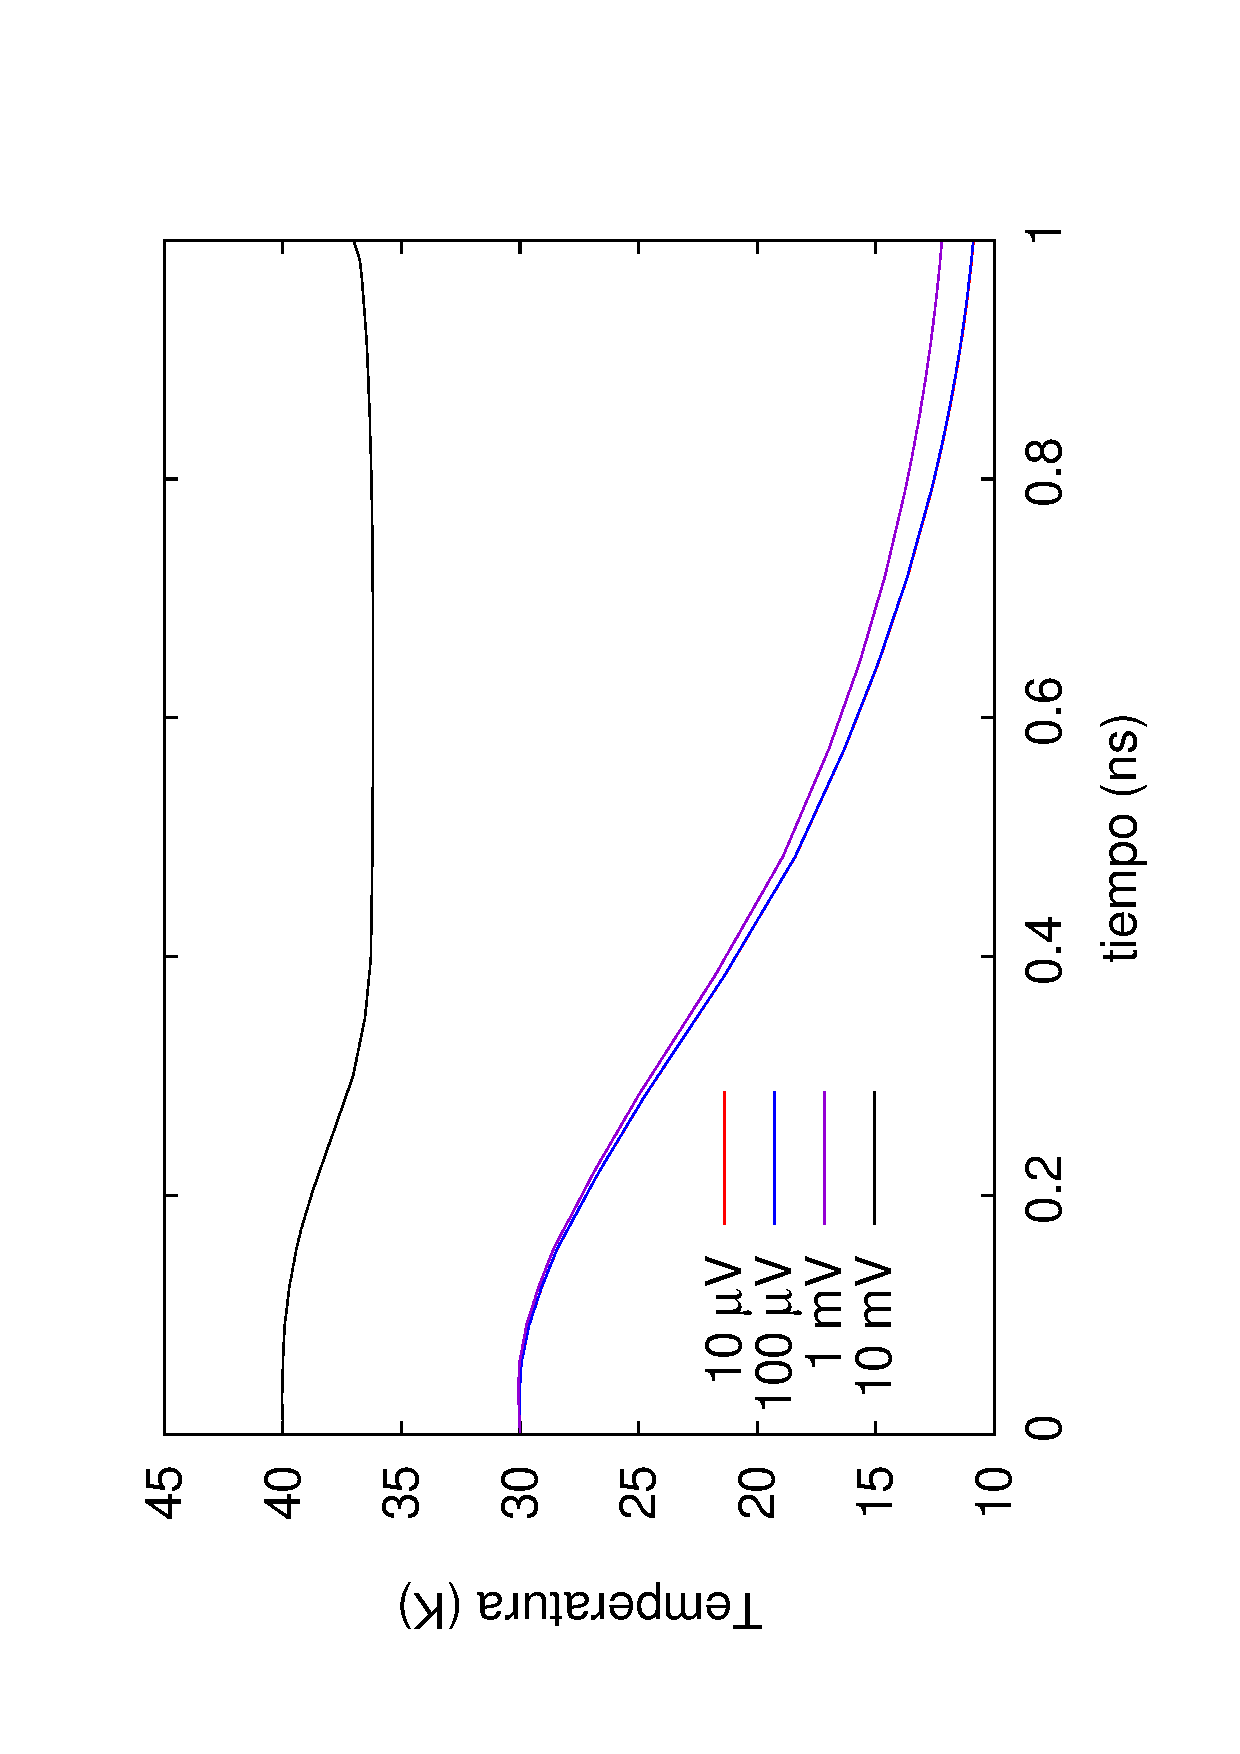
\includegraphics[width=0.95\columnwidth]{Tvst_Vest_200x1}
   \end{center}
   \caption[Estudio de la variación de la temperatura en función del tiempo para un detector operado a tensión constante, variando la tensión de operación.]{Estudio de la variación de la temperatura en función del tiempo para un detector operado a tensión constante, variando la tensión de operación. La fuente fría se mantuvo a 10\,K. Puede verse que que al incrementar la tensión la temperatura a la que estabiliza el sistema se incrementa tambi\'en.}
   \label{fig:TvstxV}
 \end{figure}

Para realizar este estudio se simuló un cable con una geometría similar a la de las secciones anteriores, analizando sólo el caso de un detector de 200\,nm de espesor. Se dispuso que la temperatura de la fuente fría fuera de 10\,K. Se eligió esta temperatura considerando que es la mínima alcanzable por un criogenerador comercial Gifford-MacMahon, que es un equipo criogénico con un costo accesible. Se propuso como condición inicial que el cable de MgB$_2$ se encontrara a una temperatura de 30 o 40\,K para luego ver cómo variaba la temperatura del mismo con el tiempo. Se realizaron simulaciones para diferentes tensiones aplicadas en bornes del cable, y en la Fig. \ref{fig:TvstxV} puede verse como, mientras la tensión aplicada es baja, el sistema siempre relaja a la temperatura de la fuente fría. Por otro lado, a una tensión del orden de 10\,mV puede verse que la producción de calor debida al efecto Joule compensa la pérdida de energía hacia la fuente fría, y el sistema logra estabilizarse a una temperatura de trabajo razonable.
%\newpage
Sin embargo, el problema que aparece ahora es que la tensión que hay que aplicar obliga al paso de corrientes enormes por el detector, como puede verse en la Fig. \ref{fig:IvstxV}. Esto indica que, aunque es en principio posible controlar la temperatura de operación simplemente variando la tensión aplicada al detector, esto implica que a través del detector circularán corrientes que son inaceptables desde el punto de vista práctico.
  \begin{figure}[tbh!]
	\begin{center}
	  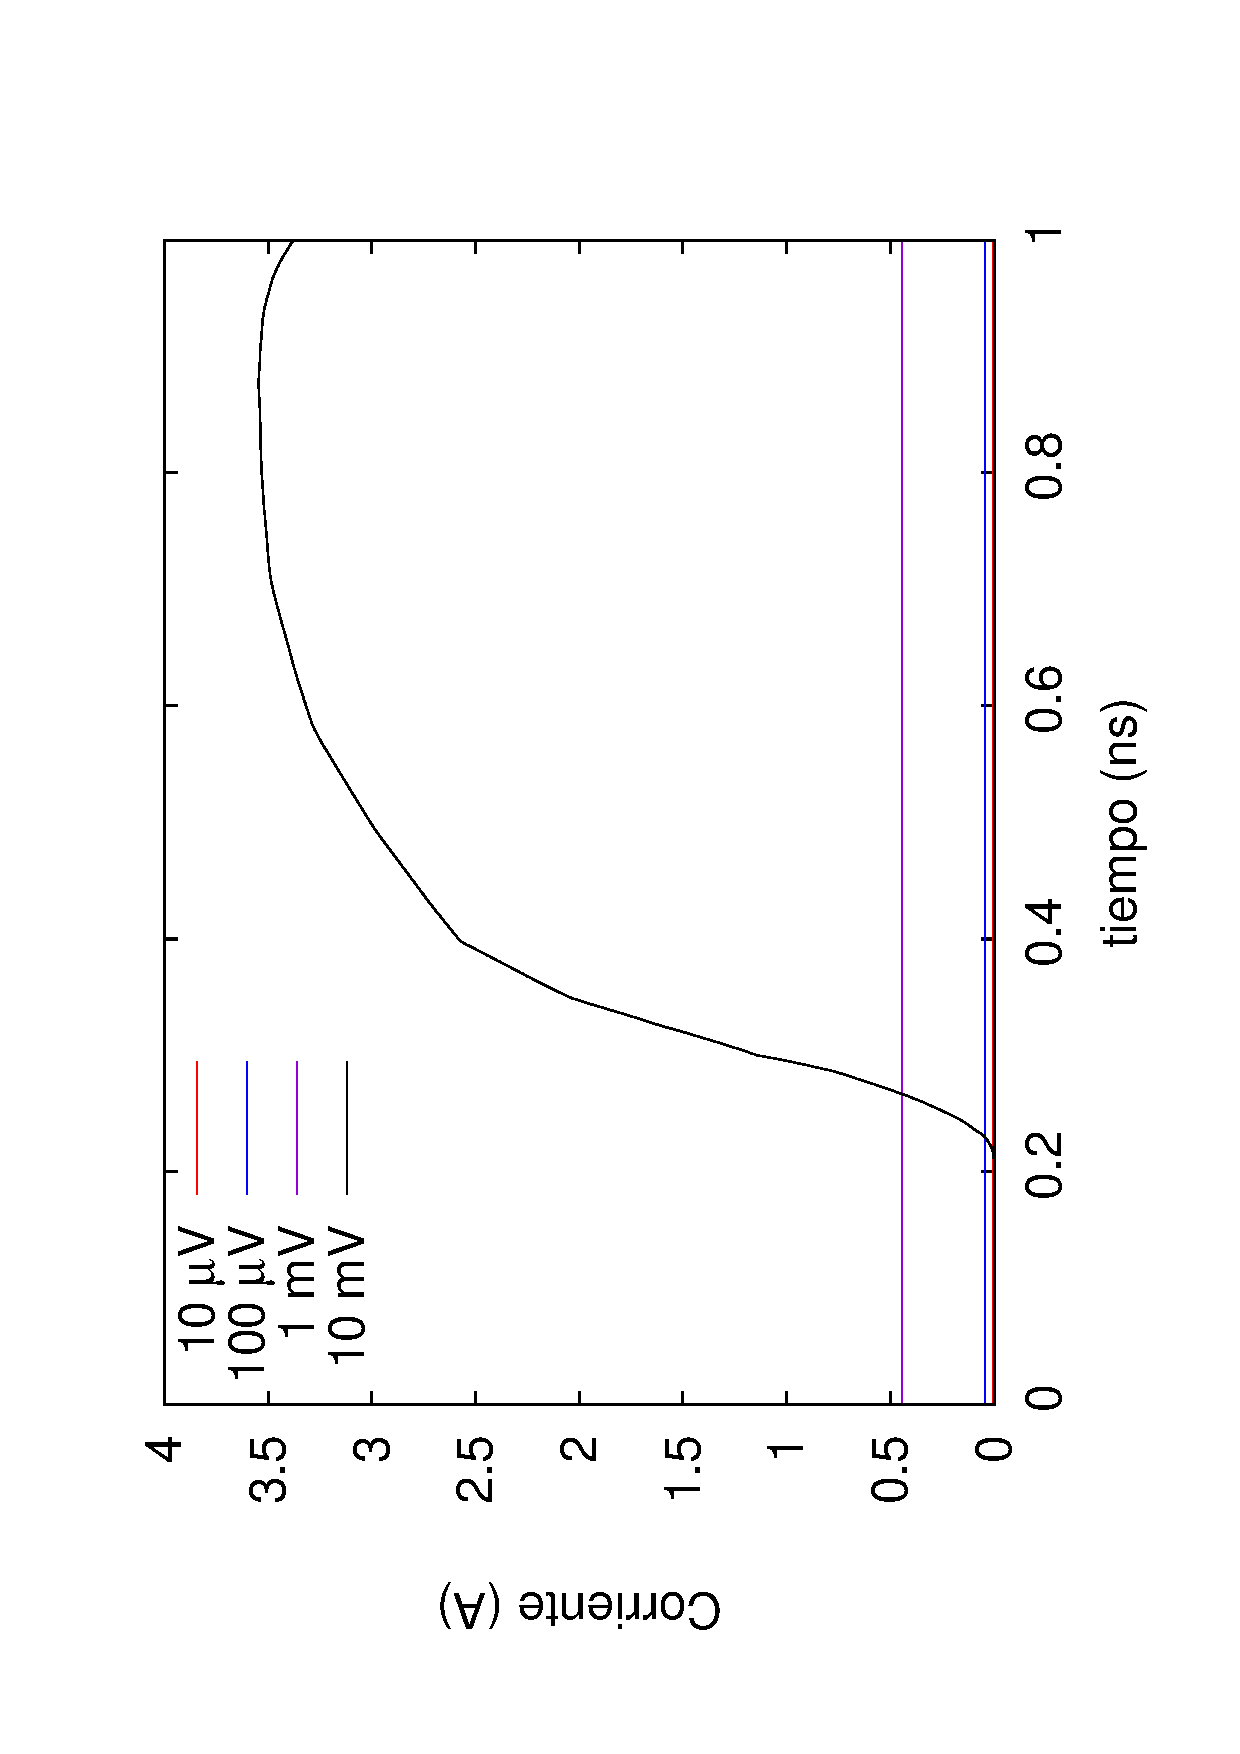
\includegraphics[width=0.55\columnwidth, angle=-90]{Ivst_200x1_Vest}
	\end{center}
	\caption[Cálculo de la corriente que circula por el detector en función de la tensión aplicada en función del tiempo.]{Cálculo de la corriente que circula por el detector en función de la tensión aplicada en función del tiempo. Como puede verse, el rango de tensiones útiles para controlar la temperatura del detector, implica el paso de grandes corrientes por el mismo. De aquí se concluyó que no es viable controlar la temperatura de operación del detector a partir de la tensión aplicada al mismo.}
	\label{fig:IvstxV}
  \end{figure}

Resulta por lo tanto, indispensable agregar un mecanismo externo para controlar la temperatura de operación del detector. Se pueden proponer dos mecanismos para lograr esto. Uno es simplemente controlar la temperatura de la fuente fría con un termómetro, un calefactor y un controlador de temperatura. También se puede pensar en depositar, entre el sustrato y el detector, algún material semiconductor que luego sea conectado a una fuente de corriente. De esta forma se implementa un mecanismo de control de temperatura utilizando la disipación Joule en el semiconductor como señal de realimentación, tal como se pretendía hacer con el propio detector.

Cabe mencionar, por último, que aunque controlar el detector con una fuente de tensión constante no sea un mecanismo viable para controlar la temperatura, sí resulta una opción atractiva por otras razones. Por un lado, al fijar la tensión y medir variaciones de corriente, se puede conseguir una buena amplificación de la señal simplemente poniendo en serie con el detector una inductancia\cite{Ishida2008}. Por otro lado tal como se explicó en la sección \ref{S:tes}, en caso de existir inhomogeneidades a lo largo del volumen del detector, si el mismo está regulado a corriente constante, el sistema se puede volver altamente inestable. Teniendo en cuenta estos detalles, es razonable concluir que el detector debe operarse a tensión constante.
\section{Eficiencia del detector}\label{S:eficiencia}
Para realizar el cálculo de la eficiencia del detector se partió de la ecuación de transmisión de neutrones para el caso de un sólo tipo de núcleo\cite{knoll}:
\begin{equation}
 \phi \ = \ \phi_0 \, e^{-n S d}
  \label{eq:t1}
\end{equation}
\noindent
siendo $\phi_0$ y $\phi$ el flujo inicial y final de neutrones, respectivamente, $n$ la densidad de núcleos por unidad de volumen, $S$ la sección eficaz total para la interacción núcleo-neutrón y $d$ el espesor de la muestra. La transmisión $\mathcal{T}$ se define como:
\begin{equation}
 \mathcal{T} \ = \ \frac{\phi}{\phi_0} \ = \ e^{-n S d}
  \label{eq:T}
\end{equation}
\noindent
Adicionalmente se puede definir el camino libre medio de un neutrón en el material considerado como la inversa del producto de la sección eficaz de interacción y la densidad la densidad de núcleos por unidad de volumen, es decir, si se nota como $\lambda_n$ al camino libre medio de un neutrón en el detector se puede escribir:
\begin{equation}
 \lambda_n \ = \ \frac{1}{n S}
  \label{eq:camino}
\end{equation}

Como $\mathcal{T}$ es la probabilidad de que un neutrón pase a través del blanco sin interactuar con el mismo, si el blanco posee diferentes tipos de núcleos, la transmisión total es simplemente el producto de las transmisividades individuales:
\begin{equation}
 \mathcal{T} \ = \ \prod _i e^{-n_i S_i d}
\label{eq:Ttot}
\end{equation}
\noindent
donde la productoria corre sobre todos los tipos de núcleos presentes. La absorción $\mathcal{A}$ indica la eficiencia del detector y se define inmediatamente a partir de la Ec.\,\ref{eq:Ttot}:
\begin{equation}
 \mathcal{A} \ = \ 1 \, - \, \mathcal{T}
\label{eq:A}
\end{equation}

El cálculo de $\mathcal{A}$ se hizo primero considerando que el superconductor fue hecho con B natural y luego con
$^{10}$B puro. Las secciones eficaces de scattering y absorción se obtuvieron de \cite{secceff}, y los valores $n_i$
de cada núcleo se obtuvieron a partir del valor de densidad teórico del MgB$_2$\cite{Lui2003} y de las distribuciones isotópicas naturales del Mg y del\,B. 

En primer lugar se calculó la eficiencia del detector suponiendo que el haz de neutrones es perpendicular al film (ver Fig.\,\ref{fig:Avsd_perpendicular}), variando el espesor del film en el rango de 0.2\,$\mu$m a 1\,$\mu$m. Si el haz incide en perpendicularmente al film se logra incrementar el área de colección a cambio de reducir el camino que debe recorrer el neutrón dentro del material. Para el caso del film hecho con B natural se calculó la absorción sumando primero las contribuciones del scattering y la absorción de todos los núcleos presentes y luego se repitió el cálculo considerando sólo la sección eficaz de absorción del $^{10}$B presente en el detector. A partir del resultado de esta cuenta se encontró que el error cometido al considerar solamente la sección eficaz de absorción del $^{10}$B en la estimación de la eficiencia del detector es menor al 1\,\%. Esto era de esperarse porque la diferencia de la sección eficaz de absorción del $^{10}$B respecto de las demás es de entre tres y cuatro órdenes de magnitud.

\begin{figure}[th!]
\vspace{-1cm}
  \begin{center}
    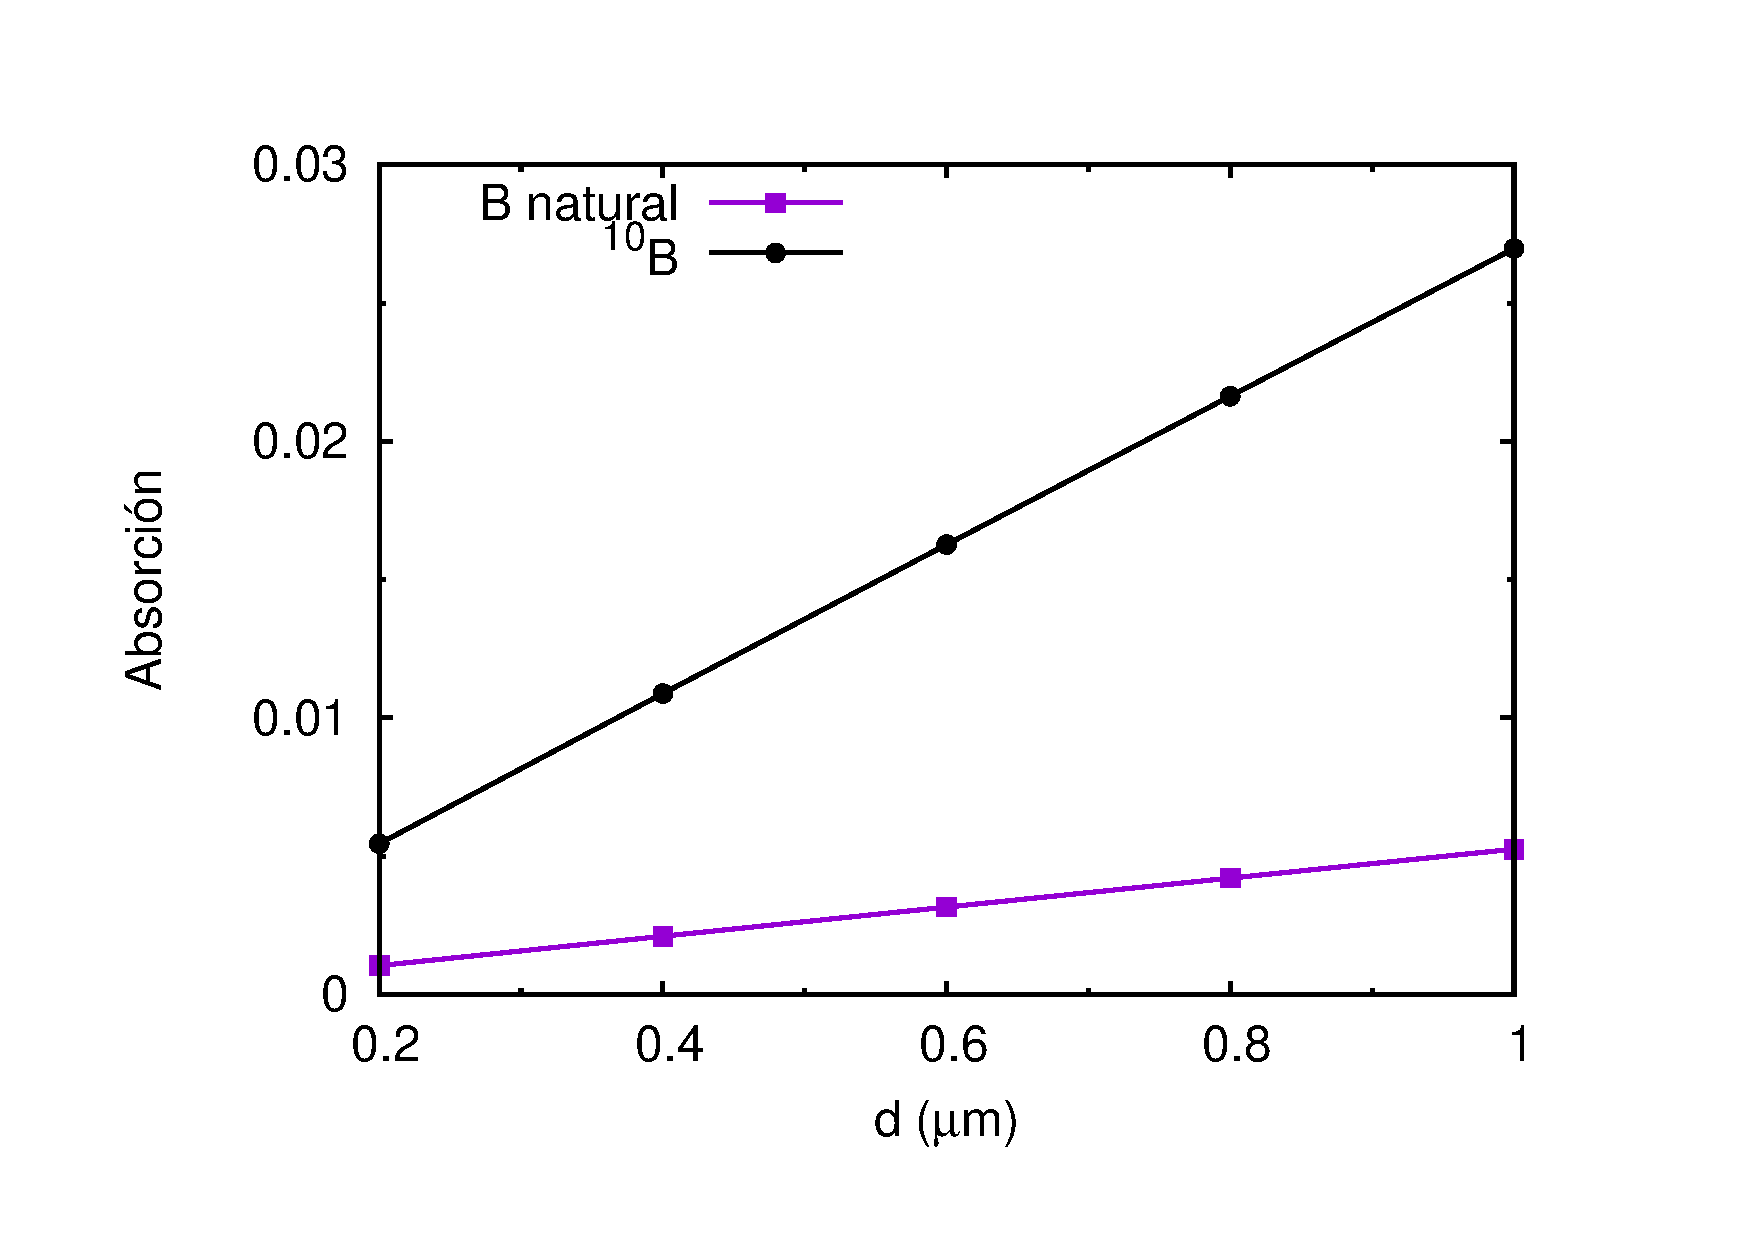
\includegraphics[width=0.9\columnwidth, angle=0]{Avsd_perpendicular}
  \end{center}
  \vspace{-1cm}
  \caption[Variación de la eficiencia del detector de MgB$_2$ en función del espesor del mismo, para un haz que incide perpendicularmente en el film.]{Variación de la eficiencia del detector de MgB$_2$ en función del espesor del mismo, para un haz que incide perpendicularmente en el film. Puede verse que la eficiencia del detector aumenta considerablemente al reemplazar el B natural del superconductor por $^{10}$B, y que es lineal con el espesor del film dentro del intervalo considerado.}
\label{fig:Avsd_perpendicular}
\end{figure}

En la Fig.\,\ref{fig:Avsd_perpendicular} se ve la variación del coeficiente de absorción de neutrones en función del espesor del detector, considerando sólo la sección eficaz de absorción del $^{10}$B. Puede observarse que la eficiencia del detector crece linealmente con el espesor del film, lo cual es razonable ya que dicho espesor es mucho menor que el camino libre medio de un neutrón en el MgB$_2$ ($\lambda_n(\rm MgB_2) \ \approx \ 35$\,$\mu$m). Se verificó además que, en este rango de espesores, la capacidad de absorción del detector se incrementa proporcionalmente con la concentración de $^{10}$B en el detector, lo que también es intuitivamente razonable.

También se calculó la eficiencia del detector suponiendo que el haz de neutrones incide en forma paralela al film de MgB$_2$, lo que supone reducir el área de colección de neutrones pero permite un incremento notable de la eficiencia, ya que ahora el neutrón debe recorrer varias veces el camino libre medio $\lambda_n$ dentro del MgB$_2$, y esto hace que la probabilidad de que ocurra la captura de un neutrón por un núcleo de $^{10}$B se vuelva próxima a 1.
\begin{figure}[h!]
 \vspace{-0.5cm}
  \begin{center}
    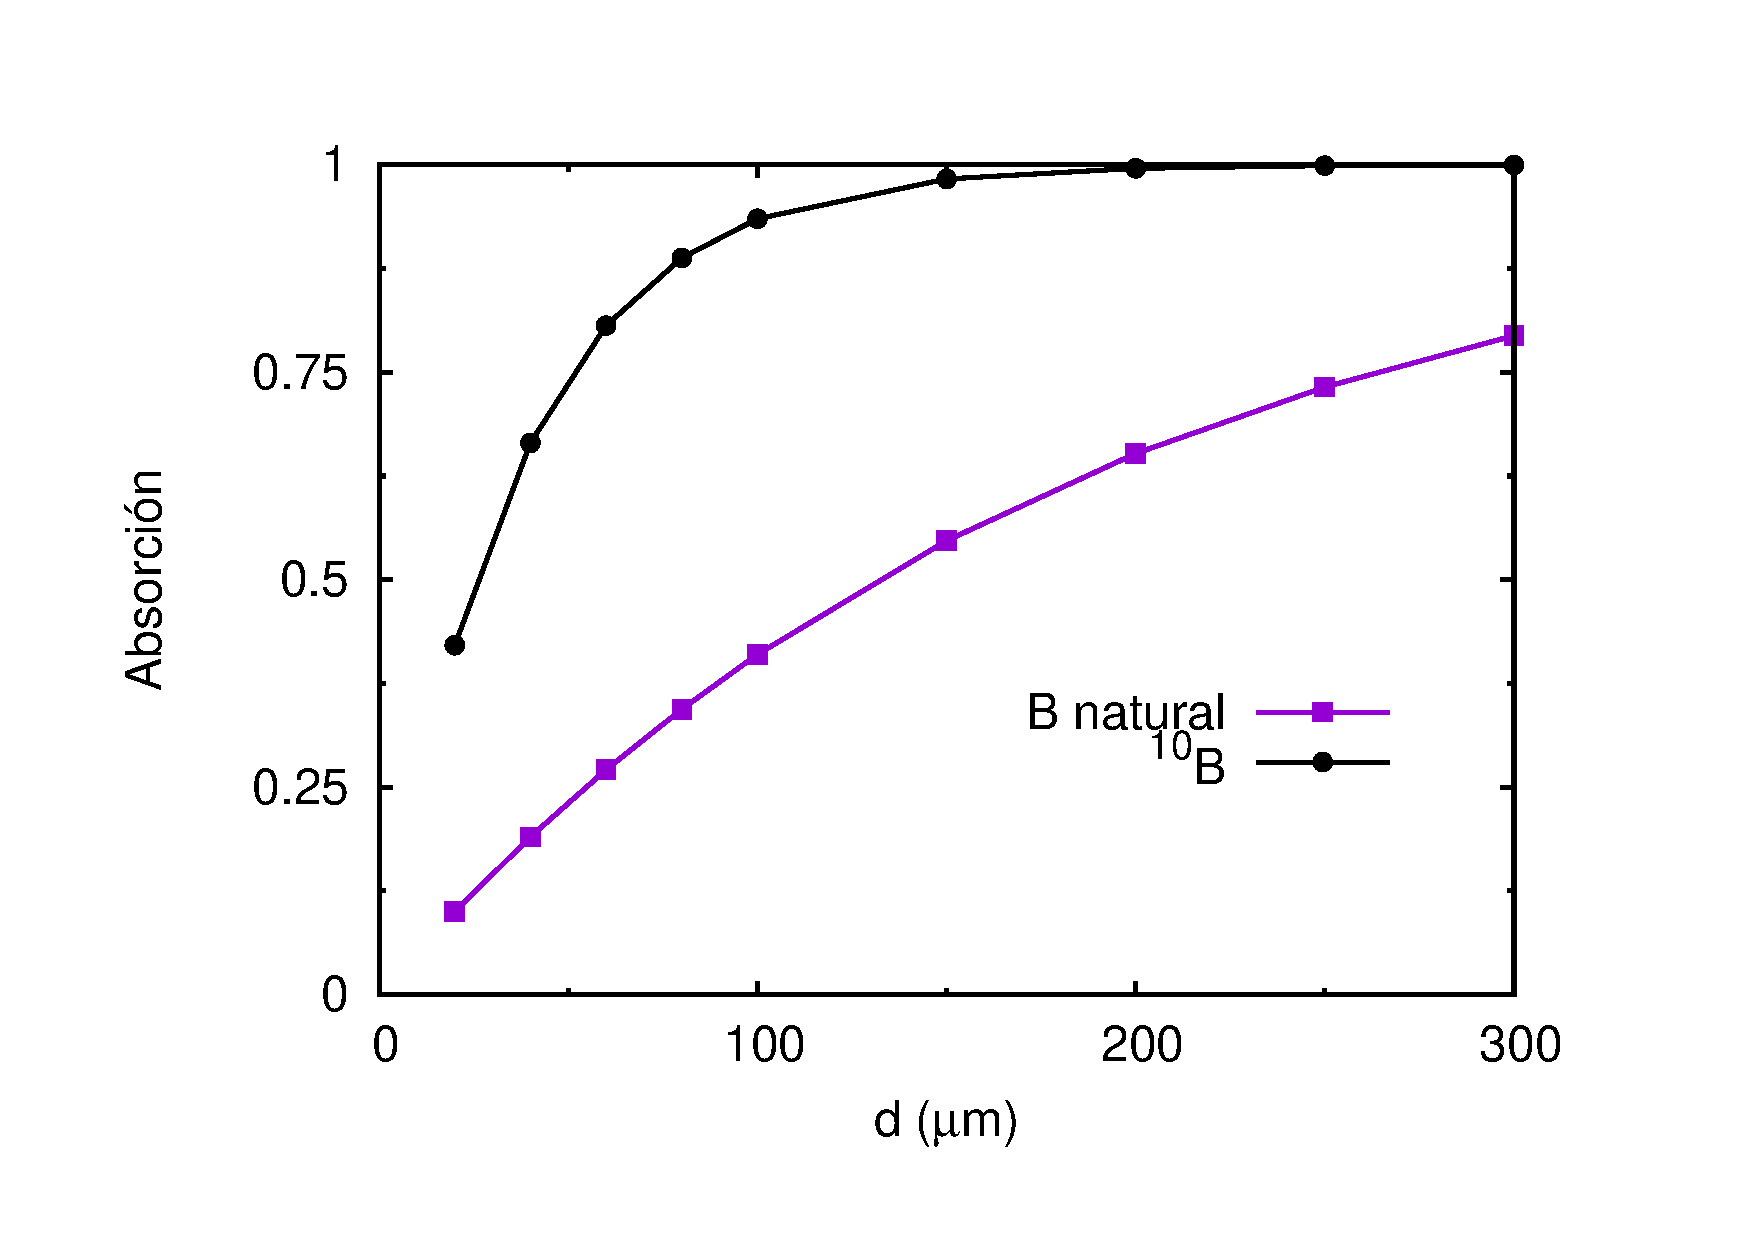
\includegraphics[width=0.9\columnwidth, angle=0]{Avsd_paralelo}
  \end{center}
  \vspace{-1cm}
  \caption[Variación de la eficiencia del detector de MgB$_2$ en función del espesor del mismo, para un haz que incide paralelamente al film.]{Variación de la eficiencia del detector de MgB$_2$ en función del espesor del mismo, para un haz que incide paralelamente al film. En esta configuración, el beneficio que se obtiene al reemplazar el B natural del superconductor por $^{10}$B es mucho menor que el observado en la Fig.\,\ref{fig:Avsd_perpendicular}, cuando el haz neutrones incidía perpendicularmente al film. También se observa que la eficiencia deja de crecer linealmente con el espesor del film y que para un cable de 300\,$\mu$m de longitud, la eficiencia del detector supera el 75\,\%.}
\label{fig:Avsd_paralelo}
\end{figure}

En la Fig.\,\ref{fig:Avsd_paralelo} pueden verse los resultados de calcular la eficiencia del detector para esta configuración.  En esta situación se observa que la eficiencia del detector es mucho mayor que para la configuración anterior y que dicha eficiencia ya no se incrementa linealmente con el espesor, todo lo cual es debido a que ahora el camino que debe recorrer el neutrón en el MgB$_2$ es comparable o mayor a $\lambda_n$. Por otro lado, al incrementarse el volumen de colección en la dirección del haz de neutrones, la eficiencia tiende a 1 y ya no se obtiene un beneficio tan notable al construir el detector utilizando únicamente $^{10}$B. Por último cabe aclarar que aunque esta configuración presenta eficiencias notablemente mayores que las mostradas anteriormente, tiene la desventaja de que permite registrar un número reducido de eventos, ya que ahora el área disponible para la colección de neutrones es muy inferior al caso anterior.

Vale la pena comentar que las eficiencias calculadas en esta sección constituyen un límite superior a la eficiencia real del detector, ya que en este modelo se está teniendo en cuenta que cada captura produce un evento en el detector, lo que no es cierto en general. Si se tiene en cuenta lo discutido en la sección \ref{S:term}, respecto a la estimación del volumen en que se deposita la energía de la reacción, y lo analizado en la sección \ref{S:signal}, respecto a las dimensiones mínimas que debe tener el cable para que se pueda obtener una buena señal a la salida del detector, debe concluirse que las eficiencias calculadas en esta sección son mayores a las efectivamente se deberían observar por lo menos en un factor 3. Esto se debe a que los fragmentos que salen en dirección perpendicular al largo del del cable de MgB$_2$ tienen muy baja probabilidad de depositar su energía en el mismo y escaparán del material.

Cabe mencionar que aunque la eficiencia de este tipo de detectores parece ser muy pobre, son del orden de las que se pueden esperar en los detectores sensibles a posición, tal como el que se planea construir. Esto es así porque cuando se quiere realizar un detector con elevada resolución espacial, es preciso que la energía del evento que se quiere detectar se deposite en una región pequeña del material, tanto más pequeña cuanto más preciso se quiere ser a la hora de definir el lugar en el que ocurrió el evento. Como la eficiencia de detección está relacionada directamente con el volumen de colección que tenga el dispositivo, es de esperar que si se busca resolución en posición, se pierda eficiencia de detección.

\nomenclature{$S$}{Sección eficaz total para la interacción entre un núcleo y un neutrón.}
\nomenclature{$n$}{Número de átomos por unidad de volumen.}
\nomenclature{$\lambda_n$}{Camino libre medio de un neutrón en un material dado.}
